\documentclass[11pt]{report}
\usepackage{acl}
\usepackage{graphicx}
\bibliographystyle{acl}
\usepackage[parfill]{parskip} 
\usepackage{alltt}
\usepackage{subfigure}
\usepackage{enumerate}

\makeatletter
\newcommand{\@BIBLABEL}{\@emptybiblabel}
\newcommand{\@emptybiblabel}[1]{}
\makeatother
\usepackage{hyperref}
\hypersetup{
    colorlinks,
    citecolor=black,
    filecolor=black,
    linkcolor=black,
    urlcolor=black
}
\usepackage[all]{hypcap}

\newcommand{\Xml}{{\sc Xml}}
\newcommand{\xml}{{\sc xml}}
\newcommand{\dtd}{{\sc dtd}}
\newcommand{\Jdk}{{\sc Jdk}}
\newcommand{\jdk}{{\sc jdk}}
\newcommand{\id}{{\sc id}}
\newcommand{\pos}{{\sc pos}}
\newcommand{\ctrl}{{\tt Ctrl+}}
\newcommand{\ctrlalt}{{\tt Ctrl+Alt+}}
\newcommand{\ctrlshift}{{\tt Ctrl+Shift+}}

\begin{document}

\title{
\textbf{English PropBank Annotation Guidelines}
 }
\author{\\
\textbf{Claire Bonial}\\
\textit{bonial@colorado.edu}\\\\
\textbf{Julia Bonn}\\
\textit{julia.bonn@colorado.edu}\\\\\
\textbf{Kathryn Conger}\\
\textit{kathryn.conger@colorado.edu}\\\\
\textbf{Jena Hwang}\\
\textit{hwangd@colorado.edu}\\\\\
\textbf{Martha Palmer}\\
\textit{mpalmer@colorado.edu}\\\\\
\textbf{Nicholas Reese}\\
\textit{nicholas.reese@colorado.edu}\\\\\
Center for Computational Language and Education Research \\
Institute of Cognitive Science \\
University of Colorado at Boulder \\\\\\
Based on original PropBank guidelines by Olga Babko-Malaya}

\maketitle
\pagebreak

\tableofcontents
\pagebreak

\chapter{Verb Annotation Instructions}
\section{PropBank Annotation Goals}
\label{ssec: Argroles}

PropBank is a corpus in which the arguments of each predicate are annotated with their semantic roles in relation to the predicate \cite{palmer-05a}.  Currently, all the PropBank annotations are done on top of the phrase structure annotation of the Penn TreeBank~\cite{marcus-93a}.  In addition to semantic role annotation, PropBank annotation requires the choice of a sense \id\ (also known as a \textit{frameset} or \textit{roleset} \id) for each predicate.  Thus, for each verb in every tree (representing the phrase structure of the corresponding sentence), we create a PropBank instance that consists of the sense \id\ of the predicate (e.g. {\tt run.02}) and its arguments labeled with semantic roles.  

\noindent An important goal is to provide consistent argument labels across different syntactic realizations of the same verb, as in\ldots

[\textit{John}]$_{ARG0}$ \textit{broke} [\textit{the window}]$_{ARG1}$ \\ \relax
[\textit{The window}]$_{ARG1}$ \textit{broke}

\noindent As this example shows, the arguments of the verbs are labeled as numbered arguments: ARG0, ARG1, ARG2, and so on.  The argument structure of each predicate is outlined in the PropBank frame file for that predicate.  The frame file gives both semantic and syntactic information about each sense of the predicate lemmas that have been encountered thus far in PropBank annotation.  The frame file also denotes the correspondences between numbered arguments and semantic roles, as this information is somewhat unique for each predicate. Each numbered argument is labeled with a semantically descriptive name, as well as a three-letter function tag taken from the list used for modifier annotation, described below. Numbered arguments reflect either the arguments that are required for the valency of a predicate (e.g., agent, patient, benefactive), or if not required, those that occur with high-frequency in actual usage.  Although numbered arguments correspond to slightly different semantic roles given the usage of each predicate, in general, numbered arguments correspond to the following semantic roles: 

\begin{table}[htp]
\centering
\begin{tabular}{|c|c||c|c|}
\hline ARG0 & agent   & ARG4 & ending point\\
\hline ARG1 & patient & ARG5 & direction, attribute\\
\hline ARG2 & instrument, benefactive, attribute, end state, extent & ARG6 & attribute\\
\hline ARG3 & starting point, benefactive, attribute   & ARGM & modifier\\
\hline 
\end{tabular}
\caption{List of arguments in PropBank}
\label{tbl:arguments}
\end{table}

\noindent In addition to numbered arguments, another task of PropBank annotation involves assigning ARGM functional tags to all modifiers of the verb, such as manner (MNR), locative (LOC), temporal (TMP) and others:

\textit{Mr. Bush met him privately, in the White House, on Thursday.} \\
REL:  met \\
ARG0: Mr. Bush \\ 
ARG1: him \\
ARGM-MNR: privately \\
ARGM-LOC: in the White House \\
ARGM-TMP: on Thursday

\noindent While these tags are used to provide semantic information about modifiers in annotation, they are also used within each frame file to provide an extra layer of semantic information about each numbered argument. Most of the numbered arguments fit neatly into one of the categories described by the function tags, with the notable exceptions of ARG0 and ARG1, which tend to correspond to agent/cause/stimulus and patient/theme/experiencer thematic roles. As these concepts will always be represented with a numbered argument in PropBank annotation, there are no corresponding tags used with modifiers that can then also be used on numbered arguments. To fill this gap in numbered argument function tagging, we have added tags called PAG and PPT, which are modeled after Dowty’s Proto-Agent and Proto-Patient roles, respectively (Dowty, 1991). A Proto-Agent is the most agent-like argument in a frame file, and a Proto-Patient is the most patient-like argument in a frame file. Since not all frame files contain an arg0, it is possible to have another numbered argument, usually ARG1, assigned a PAG function tag. Frame files are only allowed one PAG role, although those with multiple co-patient or co-theme type numbered arguments are allowed to have multiple PPT function tags. Any numbered arguments that do not fit neatly into the remaining function tag categories are assigned a tag of VSP, which denotes a Verb-SPecific role. Consider the following example of the frame file, with function tags, for  \textit{unify}:

Roleset \texttt{unify.01}, \textit{join together}:\\
ARG0-PAG: joiner, agent\\
ARG1-PPT: first (or all) thing(s) unified\\
ARG2-PPT: second thing unified\\
ARG3-VSP: unification in what domain\\
ARG4-PRD: unified whole

\noindent Finally, PropBank annotation involves finding antecedents for empty arguments of the verbs, as illustrated below:

\textit{I made a decision [*PRO*] to leave.}

\noindent The subject of the verb \textit{leave} in this example is represented as an empty category [*] in TreeBank. In PropBank, all empty categories which could be co-referred with a NP within the same sentence are linked in co-reference chains:

REL: 	leave\\
ARG0: 	[*PRO*]  * [I]

Similarly, relativizers and their referents are linked in relative clause constructions, and traces are linked to their referents in reduced relative constructions.  While these links were at one time created manually by the annotators, they are now added automatically in post-processing.  

The annotation of this information creates a valuable corpus, which can be used as training data for a variety of natural language processing applications.  Training data, essentially, is what computer scientists and computational linguists can use to `teach the computer' about different aspects of human language.  Once this information is processed, it can guide future decisions on how to categorize and/or label different features in novel utterances outside of the PropBank corpus.  Parallel PropBank corpora currently exist or are underway for English, Chinese, Arabic and Hindi.   As a whole, the PropBank corpus has the potential to assist in natural language processing applications such as machine translation, text editing, text summary and evaluation as well as question answering.  
 
 Thus, the main tasks of PropBank annotation are: argument labeling, annotation of modifiers, choosing a sense for the predicate, and creating links for empty categories, relative clauses, and reduced relatives.  Each of these aspects of annotation are discussed in detail below.  Although some detail is provided in each section on how to annotate appropriately using the annotation tool, Jubilee, complete guidelines on the use of this tool are provided in  the Jubilee technical report: \textit{Jubilee: Propbank Instance Editor Guideline (Version 2.1)} \cite{choi-09b}.
 
\section{Sense Annotation}
\subsection{Frame Files}
The argument labels for each verb are specified in the frame files, which are available at \url{http://verbs.colorado.edu/propbank/framesets-english/} and are also displayed in the frameset view of the annotation tool, Jubilee (see Jubilee technical report \cite{choi-09b} for further information).  Frame files provide verb-specific descriptions of semantic roles and illustrate these roles by providing examples. 

Frame File for the verb \textit{expect}:\\
Roles: \\
ARG0: expecter\\
ARG1: thing expected

\textbf{Example}\\
\textit{Portfolio managers expect further declines in interest rates.}

ARG0: Portfolio managers\\
REL: expect\\
ARG1: further declines in interest rates

\noindent For some verbs, it is impossible to provide one set of semantic roles for all senses of the verb. For example, the two senses of the verb \textit{leave} in the examples below take different arguments: 

\textit{Mary left the room.}\\
\textit{Mary left her daughter-in-law her pearls in her will.}

\noindent In such cases, frame files distinguish two or more verb senses, which are called framesets or rolesets (this term is interchangeable, depending on what language is being annotated), and define argument labels specific to each frameset: 

Roleset \texttt{leave.11}, \textit{depart}:\\
ARG0: entity in motion\\
ARG1: location vacated\\
ARG2: destination location

Roleset \texttt{leave.02}, \textit{give}:\\
ARG0: giver \\
ARG1: thing given\\
ARG2: beneficiary

As previously mentioned, frame files are also found in the frameset view (upper-right pane) of the annotation tool, Jubilee.  Initially, the predicate lemma followed by {\tt.XX} is displayed here to indicate that no sense has been chosen yet (e.g. {\tt leave.XX}).  

\noindent When annotating, annotators first select the appropriate roleset (or sense), and then assign the argument labels as specified for this roleset.  In Jubilee, annotators can peruse the available numbered senses of a predicate by clicking on the roleset combo-box, or they can move through the available rolesets sequentially by using the shortcut {\tt ]} to move forward, or {\tt [} to move back to lower-numbered senses.  As a roleset is selected, the argument structure and a short definition of that sense, which are extracted from the corresponding frameset file (e.g. {\tt leave.xml}), appear in the roleset information pane.   To view annotation examples of the currently selected roleset, click {\tt [Example]} button (\ctrl E). Occasionally, viewing the frameset directly on the Propbank website is beneficial to an annotator, as it may have additional notes from adjudicators on distinguishing different senses of the verb. For example, the roleset for leave.08 contains the note ``Most of these probably appear as passives. It is unclear whether benefactives can occur with the active usage. All of the active usages I've seen that appear to include the benefactive should actually be tagged as leave.01, because the 'over' is actually part of the location. ex: 'he had left the pistol over with the servants at the further side of the great tree.'" This explanatory note is also available through the {\tt[View Roleset Comments]} button or by pressing (Ctrl+C).   

\noindent To accommodate verb particle constructions (e.g. \textit{give up}) , the frame file defines not only several senses of each verb, but also several predicates reflective of the verb's associated verb particle constructions. If a verb has a particle (marked as \texttt{PRT} in TreeBank), then it is considered a different predicate, and may or may not have a different set of semantic roles. For example, the frame file for the verb \textit{keep} defines three predicates: predicate \textit{keep} (which has 6 rolesets), and predicates \textit{keep up} and \textit{keep on}, which each encompass 1 roleset respectively. The following example gives the definition of the predicate \textit{keep up} and an example usage:

\textbf{Predicate:  keep up:}\\
\texttt{keep.05}, \textit{maintain one's position}:\\
ARG0: maintainer of position\\
ARG1: relative to what

\textit{John can't keep up with Mary's rapid mood swings.}\\
ARG0: John \\
ARGM-MOD: ca \\
ARGM-NEG: n't \\
REL: keep up \\
ARG1: with Mary's rapid mood swings

Note that the relation (\texttt{rel}) in PB annotation should include both the verb and the particle. Thus, the annotator must concatenate the particle to the original relation to form a single predicate lemma, annotated with the \texttt{rel} tag.  To concatenate the particle, choose the particle node (as opposed to selecting just the particle itself) and type \ctrlshift /.  The resulting \texttt{rel} annotation will reflect the locations of both the original predicate and the concatenated particle in the annotation view; for example, {\tt 9:0,8:0-rel}. 

\subsection{ER: Error roleset}
All tokens marked as verbs in the TreeBank should be annotated in PropBank; however, rarely a token is marked as the \texttt{rel} that is not truly a verb and should not be annotated.  Because the lines between parts of speech are often fuzzy, annotators should annotate all cases of gerunds and past participles, even if they seem adjectival or nominal in usage.  However, if the token marked as a verb is not ever used grammatically as an active verb, then it should not be annotated and the \texttt{ER} roleset should be selected.  For example, \textit{collonaded} in `\textit{The collonaded house\ldots}' has been marked as a verb in the past in the TreeBank, but a web search shows that there are no attested usages of \textit{collonade} as an active verb; thus, this instance was treated as an error and marked as \texttt{ER}.  This roleset should also be selected when a verb is being used prepositionally, and therefore heads a prepositional phrase in the TreeBank.  For example, although \textit{accord} can appear as an active verb, prepositional usages such as `\textit{According to our sources\ldots}' should be marked as \texttt{ER}.  Other examples of verbs that are often used prepositionally are \textit{base} and \textit{give} in usages such as `\textit{Based on current research\ldots}' and `\textit{Given the situation\ldots}'  In each of these cases, the annotator will notice that the verb syntactically heads a prepositional phrase.  In general, \texttt{ER} should be selected for error cases where the \texttt{rel} is not a verb. 

The \texttt{ER} roleset should also be selected in the case of a TreeBank error. There are many different kinds TreeBank errors, but the following is a common one. Occasionaly, in noun annotation, there should be a \texttt{NML} node within an \texttt{NP} node, but the \texttt{NML} is missing. In some cases, the result is that constituents which should be grouped together within an \texttt{NML} would have to be tagged individually, requiring concatenation. This is not proper tagging procedure, and should not be done. In the following example, the \texttt{rel} should be contained in an \texttt{NML}, which it would be the head of. If this were done correctly, the instance would be taggable. Instead, it looks like the \texttt{rel} is not the head. This is a TreeBank error, and should be tagged as an \texttt{ER} roleset.

\begin{figure}[htbp]
\centering
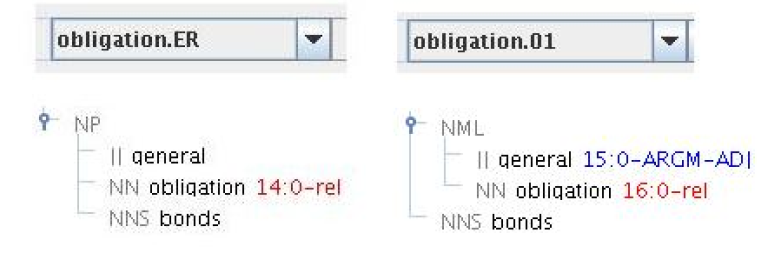
\includegraphics[scale=0.4]{img/nmler.png}
\caption{Example of a head which requires an NML node}
\label{fig: NmlEr}
\end{figure}

\subsection{IE: Idiomatic Expression roleset}
If the \texttt{rel} is part of an idiomatic expression, wherein the meaning of the expression has no relationship to the meaning of its parts, then the \texttt{IE} roleset should be selected. Because PropBank has coarse-grained senses which treat metaphorical extensions of a sense in the same manner as the literal sense, annotators should be careful not to use \texttt{IE} where the idiomatic expression is metaphorically related to the words that comprise it. For example, \textit{let} in `\textit{let the cat out of the bag}' should be annotated because `\textit{the cat}' is metaphorically related to a secret and `\textit{the bag}' is related to the secret's hidden nature. However, \textit{trip} in `\textit{Trip the light fantastic toe}' (meaning \textit{to dance}), has no relationship to dancing, and similarly, \textit{kick} in `\textit{Kick the bucket}' has no relationship to dying. In these cases, and only these cases, where the meaning of the expression is in no way related to the individual meanings of the words, the \texttt{IE} roleset should be selected. 

\subsection{DP: Duplicate indicator roleset}
This roleset is not available to annotators, but is used in post-processing to indicate that a duplicate was necessary to handle a verb that has two separate argument structures.  This occurs only in cases of verb ellipsis, for example, `\textit{I ate a sandwich and Cindy a banana}.'  The TreeBank uses special `=' notation and numbered indices to indicate that the second argument structure shares a verb given earlier. In these cases, annotators should select the appropriate numbered roleset, and should annotate only the first argument structure. Then, the annotator should fill out a problem report on the PropBank website (\url{http://verbs.colorado.edu/propbank/}), indicating that the instance needs a duplicate. During adjudication and post-processing, this duplicate is added and the second argument structure is annotated. The annotation of the second argument structure receives the \texttt{DP} roleset during post-processing so that it is clear that this instance is a duplicate.  

\subsection{LV: Light Verb roleset}
This roleset is used to flag a verb's usage as a light verb usage (e.g., \textit{take a walk, have a drink}).  See Chapter~\ref{ch: LVC} for more details on light verb annotation. 

\subsection{What to do when there is no frame file}
Occasionally, annotators will come across new verbs that do not have existing frame files. In these cases, firstly check to see if this is a mislemmatization of a verb that already has a frame file (e.g., a Britishism or misspelling). Use the frames listed on the website (\url{http://verbs.colorado.edu/propbank/framesets-english/}) to check this. If it is a mislemmatization, use the argument structure outlined in the existing frame file and take a note of the task and instance number of this problem, along with the correct roleset (e.g. \texttt{color.01}).  Using this information, fill out a problem report on the PropBank website (\url{http://verbs.colorado.edu/propbank/}). If this is not the case, the annotator will have to do some research to determine what an appropriate argument structure would be.  Brainstorm other verbs that have similar syntax and semantics, and see if any of those verbs already have frame files.  Try to model your annotation after that frame file. Again, fill out a problem report for this instance, taking note of the task and instance number along with an outline of the numbered arguments used and their semantic role correspondences. Also, include the roleset that served as a basis of comparison if one was used.  

If desired, the annotators can consult the Unified Verb Index: \url{https://verbs.colorado.edu/verb-index/}.  This has links to existing VerbNet and FrameNet information on a particular predicate, which can be used to understand what are commonly thought of as a verb's core arguments.  Where possible, PropBank is mapped to VerbNet thematic roles.  If a mapping is appropriate, a roleset's VN class will be listed at the top of the roleset on the frames website.  VerbNet uses more canonical thematic roles instead of numbered arguments that are unique to the predicate.  Thus, the annotator can use this as a resource for brainstorming argument structures for new verbs as well as coming to a better understanding of existing frame files by examining another analysis of that verb's thematic roles.  

\section{Annotation of Numbered Arguments}
\subsection{Choosing ARG0 versus ARG1}
\label{ssec: Choosing ARG0 versus ARG1}
In most cases, choosing an argument label is straightforward, given the verb specific definition of this label in the frame files. However, in some cases, it may be somewhat ambiguous whether an argument should be annotated as ARG0 or ARG1; thus, the annotator must decide between these labels based on the following explanations of what generally characterizes ARG0 and ARG1.  

The ARG0 label is assigned to arguments which are understood as agents, causers, or experiencers. The ARG1 label is usually assigned to the patient argument, i.e., the argument which undergoes the change of state or is being affected by the action. 

ARG0 arguments (which correspond to external arguments in GB theory) are the subjects of transitive verbs and a class of intransitive verbs called unergatives. Semantically, external arguments have what Dowty (1991) called Proto-Agent properties, such as:
\begin{enumerate}
\item Volitional involvement in the event or state 
\item Causing an event or change of state in another participant
\item Movement relative to the position of another participant
\cite{dowty-91}
\end{enumerate}

Internal arguments (labeled as ARG1) are the objects of transitive verbs and the subjects of intransitive verbs called unaccusatives. These arguments have Proto-Patient properties, which means that these arguments:
\begin{enumerate}
\item Undergo change of state 
\item Are causally affected by another participant 
\item Are stationary relative to movement of another participant 
\cite{dowty-91}

\end{enumerate}

Whereas for many verbs, the choice between ARG0 or ARG1 does not present any difficulties, there is a class of intransitive verbs (known as verbs of variable behavior), where the argument can be tagged as either ARG0 or ARG1.

[\textit{A bullet}]$_{ARG1}$ \textit{landed at his feet} \\ \relax
[\textit{He}]$_{ARG0}$ \textit{landed}

Arguments which are interpreted as agents should always be marked as ARG0, independent of whether they are also the ones which undergo the action.  In general, if an argument satisfies two roles, the highest ranked argument label should be selected, where 

\begin{center}
$ARG0 > ARG1 >  ARG2-5 > ARGM$
\end{center}

Given this rule, agents are ranked higher than patients. If an argument is both an agent and a patient, then ARG0 label should be selected. An example of this is the verb \textit{meet}: 

\textit{John and Mary met at a cocktail party.} \\
ARG0: John and Mary \\
REL: met \\
ARGM-LOC: at a cocktail party 


Another good example of this is the verb \textit{move}, which can have both an ARG0 (i.e. the mover) and an ARG1 (i.e. the moved), though in some cases ARG0 and ARG1 are the same:

\textit{Digital 's move into mainframes} \\
ARG0: Digital 's \\
REL: move \\
ARG2: into mainframes 

Not all ARG0s are agentive, however. There are many inanimate as well as clausal arguments which are being marked as ARG0s. These arguments are usually the ones which cause an action or a change of state.

A notion which might be useful for selecting ARG0 arguments is the notion of internally caused as opposed to externally caused eventualities, as defined in Levin and Rapapport (1995).  In internally-caused eventualities, some property inherent to the argument of the verb is responsible for bringing about the eventuality.  For agentive verbs such as \textit{play, speak}, or \textit{work}, the inherent property responsible for the eventuality is the will or volition of the agent who performs the activity. However, an internally caused eventuality need not be agentive. For example, the verbs \textit{blush} and \textit{tremble} are not agentive, but they, nevertheless, can be considered to denote internally caused eventualities, because these eventualities arise from internal properties of the arguments, typically an emotional reaction.  In contrast to internally caused verbs, verbs which are externally caused inherently imply the existence of an external cause with an immediate control over bringing about the eventuality denoted by the verb: an agent, and instrument, a natural force, or a circumstance. Thus something breaks because of the existence of some external cause; something does not break because of its own properties \cite{levin-95}.  The difference between internal and external causation is important for distinguishing ARG0s and ARG1s: the arguments which are responsible for bringing out the eventuality are ARG0s, whereas those which undergo an externally caused event are ARG1s.  

To sum up, ARG0 arguments are the arguments which cause the action denoted by the verb, either agentively or not, as well as those which are traditionally classified as experiencers, e.g., the arguments of stative verbs such as \textit{love}, \textit{hate}, \textit{fear}.  ARG1 arguments, on the other hand, are those that change due to external causation, as well as other types of patient-like arguments.

\subsection{ARGA: Secondary Agent}
\label{ssec: ARGA}

In addition to argument numbers 1-5 and modifiers, the tag `ARGA' is available.  This should be used to annotate secondary agents.  Verbs that often take secondary agents will have this specified in the roleset and a clarifying example will be provided (e.g. walk.01); however, it is possible albeit rare for other verbs to be characterized by a secondary agent.  In general, the secondary agent tag will only be used when the argument structure outlined in the roleset indicates that a proto-agent role, such as `the walker'$_{ARG0}$ for sense walk.01,  is already fulfilled, yet there is another animate agent causing the event: 

\textit{John walked his dog}\\
ARGA: John\\
REL: walked\\
ARG0: his dog

\section{Annotation of Modifiers}
The following types of modifiers are being used in PropBank:

\hyperref[ssec: COM]{COM: Comitative} \\
\hyperref[ssec: LOC]{LOC: Locative} \\
\hyperref[ssec: DIR]{DIR: Directional} \\
\hyperref[ssec: GOL]{GOL: Goal} \\
\hyperref[ssec: MNR]{MNR: 	Manner} \\
\hyperref[ssec: TMP]{TMP: Temporal} \\
\hyperref[ssec: EXT]{EXT:	Extent} \\
\hyperref[ssec: REC]{REC:	Reciprocals} \\
\hyperref[ssec: PRD]{PRD: 	Secondary Predication} \\
\hyperref[ssec: PRP]{PRP:	Purpose} \\
\hyperref[ssec: CAU]{CAU: 	Cause} \\
\hyperref[ssec: DIS]{DIS:	Discourse} \\
\hyperref[ssec: ADV]{ADV:	 Adverbials} \\
\hyperref[ssec: ADJ]{ADJ: Adjectival} \\
\hyperref[ssec: MOD]{MOD:	Modal} \\
\hyperref[ssec: NEG]{NEG:	Negation} \\
\hyperref[ssec: DSP]{DSP:    Direct Speech} \\
\hyperref[ssec: LVB]{LVB: Light Verb} \\
\hyperref[ssec: CXN]{CXN: Construction}

Note: In the sections that follow describing each type of modifier, many real examples drawn from the corpus are used.  As such, these examples contain null elements (*, PRO) and traces (*T*).  These null elements and traces often use indices, or numbers, to show the relationship between a null element and its referent.  Thus, the null element or trace may have a number listed after it, and that number is listed again next to a word or phrase.  This indicates that the two are coreferential. For more information on null elements, refer to Section~\ref{sec: null1} and Section~\ref{sec: null2}.


\subsection{Comitatives (COM)}
\label{ssec: COM}

Comitative modifiers indicate who an action was done \textit{with}.  This can include people or organizations (entities that have characteristics of prototypical agents: animacy, volition) but excludes objects, which would be considered instrumental modifiers.  Although the formal term for this modifier is `comitative,' annotators can think of this argument as `companion:' a companion to another in the action of the verb.

\textit{I sang a song with my sister.}\\
ARG0: I\\
REL: sang\\
ARG1: a song\\
ARGM-COM: with my sister

\textit{The man joined the club with his friend.}\\
ARG0: The man\\
REL: joined\\
ARG1: the club\\
ARGM-COM: with his friend

\textit{I-1 got kicked [*-1] out of the class with the bully.}\\
REL: kicked\\
ARG1: [*-1]\\
ARGM-DIR: out of the class\\
ARGM-COM: with the bully

\textit{The next morning, with a police escort, busloads of executives and their wives raced to the Indianapolis Motor Speedway.}\\
ARGM-TMP:        The next morning \\
ARGM-COM:        with a police escort\\ 
ARG0:        busloads of executives and their wives\\ 
REL:        raced \\
ARG1:        to the Indianapolis Motor Speedway

\subsection{Locatives (LOC)}
\label{ssec: LOC}

Locative modifiers indicate where some action takes place. The notion of a locative is not restricted to physical locations, but abstract locations are being marked as LOC as well; such as `[\textit{in his speech}]-(LOC) \textit{he was talking about\ldots}' 

\textit{The percentage of lung cancer deaths among the workers at the West Groton , Mass. , paper factory appears [*-1] to be the highest for [any asbestos workers]-1 studied [*-1] in Western industrialized countries , he said [0] [*T*-2] .}\\
ARG1: [*]   \\
REL: studied\\ 
ARGM-LOC: in Western industrialized countries

\textit{Areas of the factory [*ICH*-2] were particularly dusty where-1 [the crocidolite]-8 was used [*-8] [*T*-1] .}\\
ARGM-LOC:        [*T*-1]   \\
ARG1:        [*-8]   \\
REL:        used 

\textit{In his ruling , Judge Curry added an additional \$ 55 million [*U*] to the commission 's calculations.}\\
ARGM-LOC:        In his ruling\\ 
ARG0:        Judge Curry \\
REL:        added \\
ARG1:        an additional \$ 55 million [*U*] \\
ARG2:        to the commission 's calculations

\subsection{Directional (DIR)}
\label{ssec: DIR}

Directional modifiers show motion along some path. \textit{Source} modifiers are also included in this category.  However, if there is no clear path being followed, ARGM-LOC should be used instead. Thus, `\textit{walk along the road}' is a directional, but `\textit{walk around the countryside}' is a location. Directional modifiers are also used for some particles, as in `\textit{back up}.'

\textit{What sector is [*T*-46] stepping forward [*-2] to pick up the slack ? '' he asked [*T*-1] }\\
ARG1:        [*T*-46]\\   
REL:        stepping \\
ARGM-DIR:        forward\\ 
ARGM-PRP:        [*-2] to pick up the slack

\textit{That response annoyed Rep. Markey , House aides said [0] [*T*-1] , and the congressman snapped back that there had been enough studies of the issue and that it was time for action on the matter .}\\
ARG0:        the congressman \\
REL:            snapped \\
ARGM-DIR:        back \\
ARG1:        that there had been enough studies of the issue and that it was time   for action on the matter

\subsection{Goal (GOL)}
\label{ssec: GOL}

This tag is for the goal of the action of the verb.  This includes the final destination of motion verbs and benefactive arguments that receive something, or modifiers that indicate that the action of the verb was done for someone or something, or on their behalf: 

\textit {The child fed the cat for her mother.}\\
ARG0: the child\\
RELl: fed\\
ARG1: the cat\\
ARGM-GOL: for her mother

\textit{The couple translated for the Americans.}\\
ARG0: the couple\\
REL: translated\\
ARGM-GOL: for the Americans

ARGM-GOL should also be used for modifiers that indicate the final resting place or destination of motion or transfer verbs:

\textit{Workers dumped large burlap sacks of the imported material into a huge bin , poured in cotton and acetate fibers and mechanically mixed the dry fibers in a process used [*] [*] to make filters.}
ARG0: Workers \\
REL: dumped \\
ARG1: large burlap sacks of the imported material \\
ARGM-GOL: into a huge bin

\textit{We publicized to the masses our determination to fight against evil.}\\
ARG0: We\\
REL: publicized\\
ARGM-GOL: to the masses\\
ARG1: our determination to fight against evil

\textit{The walls crumbled to the ground.}\\
ARG1: The walls\\
REL: crumbled \\
ARGM-GOL: to the ground

\noindent Be careful to distinguish instances like the above example (`\textit{The walls crumbled to the ground}') from secondary predication (e.g. `\textit{he bled \textbf{to death}}'); the difference being that the above example involves motion and coming to rest.  

\noindent Many motion verbs involving a change of state, such as \textit{rise}, and \textit{fall}, already have a numbered argument for this semantic role.  Similarly, many transfer verbs, such as \textit{give}, and \textit{distribute}, already have a numbered argument for this role.  In these cases, as in all situations where we have numbered arguments that are also encompassed by ARGMs, continue to prioritize the use of the numbered argument over that of the ARGM.  

\subsection{Manner (MNR)}
\label{ssec: MNR}

Manner adverbs specify how an action is performed. For example, `\textit{works well}' is a manner. Manner tags should be used when an adverb could be an answer to a question starting with `\textit{How}?'.

\textit{Among 33 men who-4 [*T*-4] worked closely with the substance, 28 [*ICH*-1] have died -- more than three times the expected number.}\\
ARG0: [*T*-4]   \\
REL: worked \\
ARGM-MNR: closely\\ 
ARG1: with the substance

\textit{Workers dumped large burlap sacks of the imported material into a huge bin, poured in cotton and acetate fibers and mechanically mixed the dry fibers in a process used [*] [*] to make filters.}
ARG0: Workers \\
ARGM-MNR: mechanically\\ 
REL: mixed \\
ARG1: the dry fibers\\ 
ARGM-LOC: in a process used [*] [*] to make filters

In both of these sentences, the ARGM-MNR can answer the question `\textit{How?}': \\
Q: How did the 33 men work with the substance? \\
A: Closely. 

Q: How did the workers mix the dry fibers? \\
A: Mechanically.

\subsection{Temporal (TMP)}
\label{ssec: TMP}

Temporal ARGMs show when an action took place, such as `\textit{in 1987},' `\textit{last Wednesday},' `\textit{soon},' or `\textit{immediately}.' Also included in this category are adverbs of frequency (\textit{often}, \textit{always}, \textit{sometimes}, with the exception of \textit{never}, see Section~\ref{ssec: NEG} below), adverbs of duration (\textit{for a year}, \textit{in an year}), order (\textit{first}), and repetition (\textit{again})

\textit{[A form of asbestos]-2 once used [*-2] [*] to make Kent cigarette filters has caused a high percentage of cancer deaths among a group of workers exposed [*] to it more than 30 years ago , researchers reported [0] [*T*-1] .}\\
ARG1: [*-2]   \\
ARGM-TMP: once\\ 
REL: used \\
ARG2: [*] to make Kent cigarette filters

\textit{Four of the five surviving workers have asbestos-related diseases, including three with recently diagnosed cancer.}\\
ARGM-TMP: recently \\
REL: diagnosed \\
ARG2: cancer 

 \subsection{Extent (EXT)}
\label{ssec: EXT}

ARGM-EXTs indicate the amount of change occurring from an action, and are used mostly for the following: 
\begin{enumerate}
\item Numerical adjuncts, `\textit{raised prices \textbf{by 15 percent}}'
\item Quantifiers such as \textit{a lot}, \textit{least}, \textit{incredibly}, \textit{extremely}, or \textit{really}
\item Comparatives, `\textit{he raised prices \textbf{more than she did}}' 
\end{enumerate}

\textit{PS of New Hampshire shares closed yesterday at \$ 3.75 [*U*], off 25 cents, in New York Stock Exchange composite trading.}\\
ARG1:        PS of New Hampshire shares\\ 
REL:        closed \\
ARGM-TMP:        yesterday\\ 
ARGM-EXT:        at \$ 3.75 [*U*], off 25 cents, \\
ARGM-LOC:        in New York Stock Exchange composite trading 

\textit{`An active 55-year-old in Boca Raton may care more about Senior Olympic games, while a 75-year-old in Panama City may care more about a seminar on health,' she says [*T*-1].}\\
ARG0:        An active 55-year-old in Boca Raton\\ 
ARGM-MOD:        may \\
REL:       	 care \\
ARGM-EXT:        more\\ 
ARG1:        about Senior Olympic games\\ 
ARGM-ADV: while a 75 year old in Panama City may care more about a seminar on health

\textit{Rep. Jerry Lewis , a conservative Californian , added a provision of his own, intended [*] to assist Bolivia, and the Senate then broadened the list further by [*-1] including all countries in the U.S. Caribbean Basin initiate as well as the Philippines - [*-1] backed [*] by the powerful Hawaii Democrat Sen. Daniel Inouye.}\\
ARG0:        the Senate \\
ARGM-TMP:        then \\
REL:        broadened \\
ARG1:        the list \\
ARGM-EXT:        further \\
ARGM-MNR:        by [*-1] including all countries in the U.S. Caribbean Basin initiate as well as the Philippines \\
ARGM-PRD:        [*-1] backed [*] by the powerful Hawaii Democrat Sen. Daniel Inouye 

\subsection{Reciprocals (REC)}
\label{ssec: REC}

These include reflexives and reciprocals such as \textit{himself}, \textit{itself}, \textit{themselves}, \textit{each other}, or \textit{own}, which refer back to one of the other arguments. Often, these arguments serve as the ARG1 of the relation. In these cases, the argument should be annotated as the numbered argument as opposed to the reciprocal modifier. 

\textit{But voters decided that if the stadium was such a good idea someone would build it himself, and rejected it 59\% to 41\% [*U*].}\\
ARGM-ADV:        if the stadium was such a good idea \\
ARG0:        someone \\
ARGM-MOD:        would \\
REL:        build \\
ARG1:        it \\
ARGM-REC:        himself 

\subsection{Secondary Predication (PRD)}
\label{ssec: PRD}

These are used to show that an adjunct of a predicate is in itself capable of carrying some predicate structure. 

Typical examples include:
\begin{enumerate}
\item Resultatives, `\textit{The boys pinched them \textbf{dead}' or `She kicked [the locker lid]-1 [*-1] \textbf{shut}}' 
\item Depictives, `\textit{\textbf{Rosy-cheeked}, Santa came down the chimney}' 
\item As-phrases, `\textit{supplied \textbf{as security in the transaction}}' 
\end{enumerate}

In each of these cases, it is notable that the argument labeled PRD modifies another argument of the verb (describing its state during or after the event) more than it modifies the verb or event itself.  

\textit{Pierre Vinken , 61 years old , will join the board as a nonexecutive director Nov. 29 .}\\
ARG0:        Pierre Vinken , 61 years old , \\
ARGM-MOD:        will \\
REL:        join \\
ARG1:        the board\\ 
ARGM-PRD:        as a nonexecutive director\\ 
ARGM-TMP:        Nov. 29 

\textit{Prior to his term , a teacher bled to death in the halls , [*-1] stabbed [*-2] by a student.}\\
ARGM-TMP:        Prior to his term \\
ARG1:        a teacher \\
REL:        bled \\
ARGM-PRD:        to death\\ 
ARGM-LOC:        in the halls\\ 
ARGM-ADV:        [*-1] stabbed [*-2] by a student

\textit{This wage inflation is bleeding the NFL dry, the owners contend [*T*-1]. }\\
ARG0:        This wage inflation \\
REL:        bleeding \\
ARG1:        the NFL \\
ARGM-PRD:        dry 

\subsection{Purpose Clauses (PRP)}
\label{ssec: PRP}

Purpose clauses are used to show the motivation for some action. Clauses beginning with `\textit{in order to}' and `\textit{so that}' are canonical purpose clauses.

\textit{More than a few CEOs say [0] the red-carpet treatment tempts them to return to a heartland city for future meetings.}\\
ARG1:        them \\
REL:        return \\
ARG4:        to a heartland city\\ 
ARGM-PRP:        for future meetings

\textit{In a disputed 1985 ruling , the Commerce Commission said [0] Commonwealth Edison could raise its electricity rates by \$ 49 million [*U*] [*-1] to pay for the plant.}\\
ARG0:        Commonwealth Edison \\
ARGM-MOD:        could \\
REL:        raise \\
ARG1:        its electricity rates\\ 
ARG2:        by \$ 49 million [*U*]\\ 
ARGM-PRP:        [*-1] to pay for the plant

\subsection{Cause Clauses (CAU)} 
\label{ssec: CAU}

Similar to purpose clauses, these indicate the reason for an action. Clauses beginning with `\textit{because}' or `\textit{due to}' are canonical cause clauses.  Questions starting with `\textit{Why},' which are always characterized by a trace linking back to this question word, are always treated as cause. However, in these question phrases it can often be difficult or impossible to determine if the `\textit{why}' truly represents purpose or cause.  Thus, as a general rule, if the annotator cannot determine whether an argument is more appropriately purpose or cause, cause is the default choice.  

\textit{Pro-forma balance sheets clearly show why-1 Cray Research favored the spinoff [*T*-1] .}\\
ARGM-CAU:        [*T*-1]  \\
ARG0:        Cray Research \\
REL:        favored \\
ARG1:        the spinoff

\textit{However , five other countries -- China , Thailand , India , Brazil and Mexico -- will remain on that so-called priority watch list because of an interim review , U.S. Trade Representative Carla Hills announced [0] [*T*-1] .}\\
ARGM-DIS:        However \\
ARG1:        five other countries -- China , Thailand , India , Brazil and Mexico -- \\
ARGM-MOD:        will \\
REL:        remain \\
ARG3:        on that so-called priority watch list \\
ARGM-CAU:        because of an interim review 

\subsection{Discourse (DIS)}
\label{ssec: DIS}

These are markers which connect a sentence to a preceding sentence. 
Examples of discourse markers are: \textit{also}, \textit{however}, \textit{too}, \textit{as well}, \textit{but}, \textit{and}, \textit{as we've seen before}, \textit{instead}, \textit{on the other hand}, \textit{for instance}, etc.  Additionally, vocatives wherein a name is spoken (e.g. `\textit{\textbf{Alan}, will you go to the store?}') and interjections (e.g. `\textit{\textbf{Gosh}, I can't believe it}') are treated as discourse modifiers.  Because discourse markers add little or no semantic value to the phrase, a good rule of thumb for deciding if an element is a discourse marker is to think of the sentence without the potential discourse marker.  If the meaning of the utterance is unchanged, it is likely that the element can be tagged as discourse.  

Note that conjunctions such as \textit{but}, \textit{or}, and \textit{and} are only marked in the beginning of the sentence.  Additionally, items that relate the instance undergoing annotation to a previous sentence such as \textit{however}, \textit{on the other hand}, \textit{also}, and \textit{in addition}, should be tagged as ARGM-DIS.  However, these elements can alternately be tagged as ARGM-ADV when they relate arguments within the clause being annotated (e.g. `\textit{Mary reads novels in addition to writing poetry}') as opposed to relating to or juxtaposing an element within the sentence to an element outside the sentence (e.g. `\textit{In addition, Mary reads novels}').  Often, but not always, when these elements connect the annotation instance to a previous sentence, they occur at the beginning of the instance.  Consider these examples to clarify this difference:

\textit{But for now , they 're looking forward to their winter meeting -- Boca in February.}\\
ARGM-DIS:        But \\
ARGM-TMP:        for now\\ 
ARG0:        they \\
REL:        [looking] [forward] \\
ARG1:        to their winter meeting -- Boca in February 

\textit{The notification also clarifies the requirements of the evaluation.}\\
ARG0: The notification\\
ARGM-DIS: also\\
REL: clarifies
ARG1: the requirements of the evaluation.

\textit{The notification recognizes the company and also clarifies the requirements of the evaluation.}\\
ARG0: The notification\\
ARGM-ADV: also\\
REL: clarifies\\
ARG1: the requirements of the evaluation.

\noindent Remember, do not mark \textit{and}, \textit{or}, or \textit{but} when they connect two clauses in the same sentence.

\noindent As previously mentioned, another type of discourse marker includes vocatives, which are marked as VOC in TreeBank:

\textit{TreeBank annotation:}
\begin{verbatim}
 (S (NP-VOC Kris),
     (NP-SBJ *)
     (VP go
         (ADVP-DIR home)))
\end{verbatim}

\textit{PropBank annotation:}\\
ARGM-DIS: 	Kris\\
REL:		go\\
ARG0:		[*]\\
ARGM-DIR:	home

Vocative NPs in imperative sentences as shown above should not be tagged as coreference chains  (e.g. ARG0: [*] * [Kris]) in order to make annotation consistent with other examples of vocative NPs, which do not include traces: 

\textit {I ain't kidding you, Vince}\\
ARGM-DIS: 	Vince\\
REL:		kidding\\
ARG0:		I\\
ARG1:		you\\
ARGM-NEG:	n't

And, finally, the class of discourse markers includes interjections such as \textit{oh my god}, \textit{ah}, and \textit{damn}. 

\textit{I might point out that your inability to report to my office this morning has not ah limited my knowledge of your activities as you may have hoped.}\\
ARGM-DIS: ah\\
REL:	limited\\
ARGM-NEG: not\\
ARG1:	my knowledge of your activities\\
ARG0:	your inability to report to my office this morning\\
ARGM-ADV: as you may have hoped

\subsection{Modals (MOD)}
\label{ssec: MOD}

Modals are: \textit{will}, \textit{may}, \textit{can}, \textit{must}, \textit{shall}, \textit{might}, \textit{should}, \textit{could}, and \textit{would}.  These elements are consistently labeled in the TreeBank as \texttt{MOD}.  These are one of the few elements that are selected and tagged directly on the modal word itself, as opposed to selecting a higher node that contains the lexical item.  

\subsection{Negation (NEG)}
\label{ssec: NEG}

This tag is used for elements such as \textit{not},  \textit{n't}, \textit{never}, \textit{no longer}, and other markers of negative sentences. Negation is an important notion for PropBank annotation; therefore, all markers which indicate negation should be marked as ARGM-NEG. For example, when annotating adverbials like \textit{never}, which could be marked as either TMP or NEG, the NEG tag should be used.  These are also elements that are tagged directly on the lexical item itself as opposed to on a higher node.  Be careful to distinguish these from the conjunction \textit{not only}, which does not actually indicate that the verb is negative and should not be annotated because it is a conjunction.

\subsection{Direct Speech (DSP)}
\label{ssec: DSP}

A verb of expression is any verb which has a speaker/thinker argument (ARG0) and the utterance/thought (ARG1).  If the utterance is a constituent, then there is a trace in TreeBank which is coindexed with that constituent. PropBank annotation tags the trace as ARG1 in this case:

\textit{TreeBank Annotation:}
\begin{verbatim}
(S ``
     (S-TPC-1 (NP-SBJ We)
              (VP will
                  (VP win)))
     ,
     ''
     (NP-SBJ Mary)
     (VP said
         (S *T*-1))
     .))
\end{verbatim}

\textit{PropBank Annotation:}\\
REL: said\\
ARG1:  [*T*-1]\\ 
ARG0: Mary

Unfortunately, in many examples, the utterance does not correspond to one constituent in TreeBank:  

\textit{Among other things , they said  [*?*] , Mr. Azoff would develop musical acts for a new record label.}

\textit{TreeBank Annotation:}
\begin{verbatim}
(S 
    (PP (IN Among) 
      (NP (JJ other) (NNS things) ))
    (PRN 
      (, ,)
      (S 
        (NP-SBJ (PRP they) )
        (VP (VBD said) 
          (SBAR (-NONE- 0) 
            (S (-NONE- *?*) ))))
      (, ,) )
    (NP-SBJ (NNP Mr.) (NNP Azoff) )
    (VP (MD would) 
      (VP (VB develop) 
        (NP 
          (NP (JJ musical) (NNS acts) )
          (PP (IN for) 
            (NP (DT a) (JJ new) (NN record) (NN label) )))))
    (. .) )
\end{verbatim}

\noindent As the example above shows, in such cases, the ARG1 argument of the verb say is a \texttt{*?*} empty category, which does not have an index in TreeBank. PropBank annotation tags this empty category as ARG1 in this case; however, it also provides a link between this empty category and the top \texttt{S} node, which contains the utterance as well as the verb of saying. This is a rare exception wherein the annotation will include embedded arguments.  Thus, the annotator first selects and tags the entire \texttt{SBAR} node as ARG1.  Next, the annotator selects the empty trace itself \texttt{NONE-*?*} and annotates this node as ARGM-DSP.  While this annotation is still in the Jubilee memory, the annotator subsequently selects the S-node containing the \texttt{rel} and uses the \texttt{*} link to link the two together: click {\tt Argument} on the Jubilee menu bar followed by clicking {\tt Functions}.  From the options therein, select \texttt{*} (shortcut: \texttt{Ctrl+Shift+8}).  Although seasoned annotators should feel uncomfortable creating embedded, recursive annotations such as this, there is special post-processing for these cases that effectively removes what is often a \texttt{PRN} (parenthetical) node containing the relation and its arguments from the argument that is semantically `\textit{what is spoken}.'   In the final version of the PropBank, ARGM-DSP tag will be replaced by LINK-DSP, to indicate that this is not a modifier of the verb, but simply additional information about one of its arguments. Figure~\ref{fig: dsp} shows the correct annotation of an instance of DSP as it will be seen in Jubilee. 

ARG1:      [SBAR (-NONE- 0) S (-NONE- *?*)]\\
ARG0:       they\\
ARGM-DSP: [-NONE-*?*] * [Among other things , they said  [*?*] , Mr. Azoff would develop musical acts for a new record label]\\    
REL:        said

\begin{figure}[htbp]
\centering
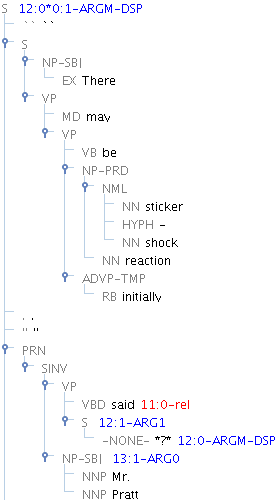
\includegraphics[scale=0.35]{img/DSPPic.png}
\caption{Correct annotation of DSP}
\label{fig: dsp}
\end{figure}

\subsection{Adverbials (ADV)}
\label{ssec: ADV}

These are used for syntactic elements which clearly modify the event structure of the verb in question, but which do not fall under any of the headings above.  The annotator should always try to use one of the alternate modifiers listed above before assuming that a modifier is merely adverbial.  However, adverbial elements are often\ldots 
\begin{enumerate}
\item Temporally related (modifiers of events): \textit{Treasures are just lying around, \textbf{waiting to be picked up}} 
\item Intensional (modifiers of propositions): \textit{probably}, \textit{possibly} 
\item Focus-sensitive \textit{only}, \textit{even} 
\item Sentential (evaluative, attitudinal, viewpoint, performatives): \textit{fortunately}, \textit{really}, \textit{legally}, \textit{frankly speaking}, clauses beginning with \textit{given that}, \textit{despite}, \textit{except for}, or \textit{if}
\end{enumerate}

As opposed to ARGM-MNR, which modify the verb,  ARGM-ADVs usually modify the entire sentence. In some cases,  modifiers like \textit{happily} can be ambiguous between MNR and ADV interpretations, as shown below: 

\textit{She sang happily.}\\
ARGM-MNR:	happily

\textit{Happily, she sang.} (paraphrase: `\textit{I am happy that she sang}')\\
ARGM-ADV:	happily

In these cases, use context as much as possible to try to make the best judgment.  

\subsection{Adjectival (ADJ)}
This tag is used in a manner that is similar to ADV, but its use is restricted to noun annotation.  See Chapter~\ref{chap: Noun Annotation Instructions} and Section~\ref{ssec: ADJ} for more details.  

\subsection{Light Verb (LVB)}
\label{ssec: LVB}

This tag is used to label the light verb only in the noun pass of light verb annotation.  See Chapter~\ref{ch: LVC} for more details.  

\subsection{Construction (CXN)}
\label{ssec: CXN}

This tag is used to label arguments that are projected by a construction, such as the comparative construction (e.g. \textit{She is taller than her sister}), as opposed to a lexical relation.  Although constructions can project arguments with a variety of lexical relations, this tag is currently only used in the annotation of adjective relations.  See Chapter~\ref{ch: ADJ Annotation} for more details. 

\section{Span of Annotation}
\label{sec: span}
For the purposes of PropBank annotation, annotators should only assign arguments within a certain syntactic span surrounding the \texttt{rel}.  The structure of the tree reflects which constituents in an utterance are truly arguments of a particular predicate; thus, even when annotators feel that a constituent outside of this span has some semantic bearing on the \texttt{rel}, it should not be annotated.  Rather, the syntactic span of annotation should be respected: everything within that span should be encompassed by an argument label (with exceptions described below), and nothing outside of that span should be annotated (with exception of linking annotation, such as that of relative clauses). 

Do not tag determiners (labeled \texttt{DT} in TreeBank) or conjuctions (labeled \texttt{CC} or \texttt{CONJP} in TreeBank), unless these begin the sentence and are being used in a discourse function, as described in Section~\ref{ssec: DIS}.  Do not tag auxiliary verbs such as \textit{have}, \textit{be}, or \textit{do}; the auxiliary verb itself will come up for annotation and at that point the auxiliary sense will  be selected without further annotation. 

Tag all and only the following:
\begin{enumerate}
\item Sisters of the verb 
\item Sisters of the VP
\end{enumerate}

To determine the span of annotation, locate the \texttt{rel} and the accompanying TreeBank tag indicating one of the following types of verbs \footnote{For a complete listing of TreeBank tags, see \url{http://bulba.sdsu.edu/jeanette/thesis/PennTags.html}}: 

\begin{tabular}{ll}
	VB & Verb, base form \\
	VBD	& Verb, past tense \\
	VBG	& Verb, gerund or present participle \\
	VBN	& Verb, past participle \\
	VBP	& Verb, non-3rd person singular present \\
	VBZ	& Verb, 3rd person singular present
\end{tabular}

Figure~\ref{fig:VBArrow} shows the TreeBank view of a typical instance in Jubilee, with the \texttt{VB} node indicated. 

\begin{figure}[htbp]
\centering
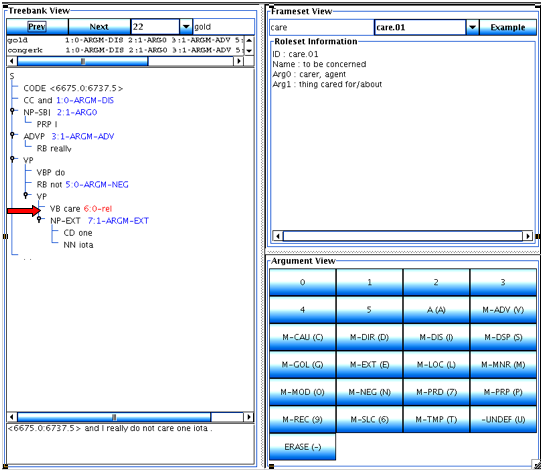
\includegraphics[scale=0.4]{img/VBArrow.png}
\caption{Find the \texttt{rel}}
\label{fig:VBArrow}
\end{figure}

Once this has been located, annotate the sisters of this node.  Sisters to the verb will be parallel to it in the tree.  Figure~\ref{fig:sisterArrow} has an arrow where the annotator should look, beginning at the verb, for sisters.  In this case, it is a relatively short distance and only the \texttt{NP-EXT} node needs to be annotated as ARG1; however, in some cases, the annotator will have to scroll up and down through Jubilee's TreeBank view to annotate multiple sisters to the verb. 

\begin{figure}[htbp]
\centering
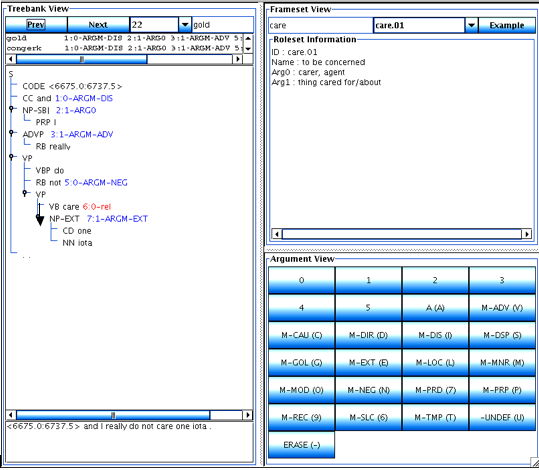
\includegraphics[scale=0.4]{img/sisterArrow.png}
\caption{Find and annotate any sisters to the \texttt{rel}}
\label{fig:sisterArrow}
\end{figure}

Next, examine the tree to see if the \texttt{VB} node is embedded in a \texttt{VP} (verb phrase) node. The verb is usually located inside a higher \texttt{VP} node, unless it is located inside an \texttt{NP} (noun phrase) node.  Where the verb is accompanied by one or more auxiliaries, it may be encompassed by several \texttt{VP} nodes, as illustrated by Figure~\ref{fig:VPArrows}, which indicates each of the \texttt{VP} nodes: 

\begin{figure}[htbp]
\centering
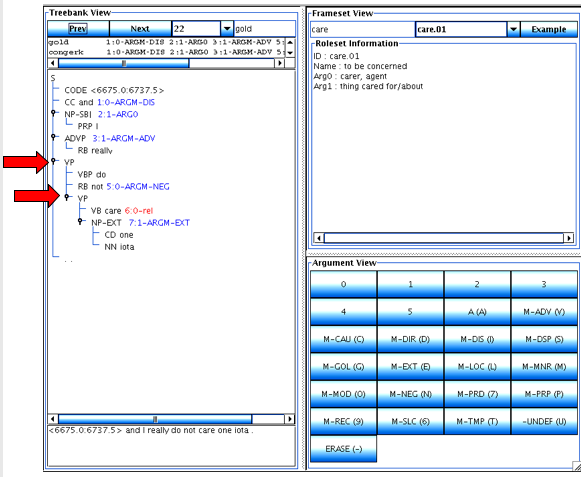
\includegraphics[scale=0.4]{img/VPArrows.png}
\caption{Find the highest \texttt{VP} node containing the \texttt{rel}}
\label{fig:VPArrows}
\end{figure}

Once the annotator has located the highest \texttt{VP} node, annotate all sisters to each \texttt{VP} node (again, the nodes that are parallel to \texttt{VP} nodes in the tree). Figure~\ref{fig:spanArrows} uses arrows to illustrate where the annotator should look, beginning at the verb, for sisters to the \texttt{VP} nodes: 

\begin{figure}[htbp]
\centering
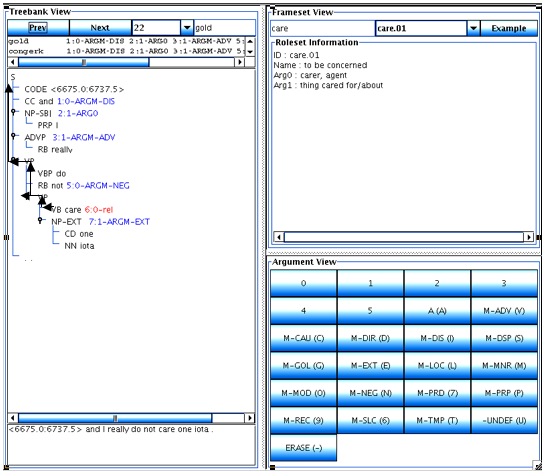
\includegraphics[scale=0.4]{img/spanArrows.png}
\caption{Find and annotate any sisters to the \texttt{VP} nodes containing the \texttt{rel}}
\label{fig:spanArrows}
\end{figure}

Thus, following this line, the annotator discovers several nodes that must be annotated: firstly, the \texttt{RB} node as ARGM-NEG; the auxiliary \textit{do} can be ignored; second, the \texttt{ADVP} node as ARGM-ADV; next the \texttt{NP-SBJ} node as ARG0; finally the \texttt{CC} node as ARGM-DIS because it meets the conditions described in Section~\ref{ssec: DIS} for serving a discourse function. The \texttt{CODE} node can be ignored when present.  Additionally, \texttt{TOP} nodes at the very top of an instance should never be annotated.  

The last thing to note is that when the verb is embedded in a \texttt{VP} node, `\textit{\texttt{S} marks the spot}' to stop annotation: 

\begin{figure}[htbp]
\centering
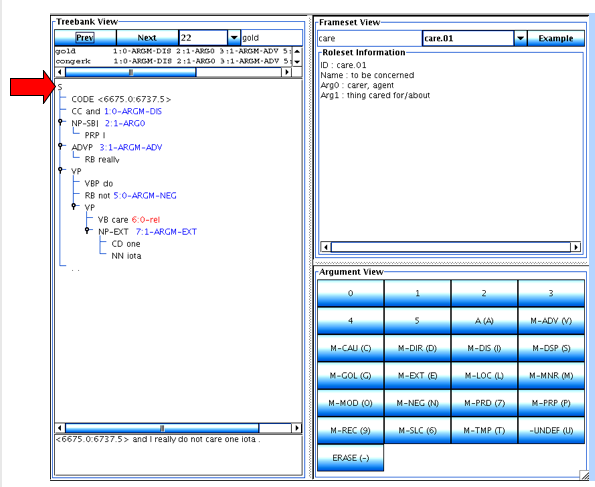
\includegraphics[scale=0.4]{img/SArrow.png}
\caption{Stop at \texttt{S}}
\label{fig:SArrow}
\end{figure}

\texttt{S} indicates clausal boundaries in the TreeBank. Thus, anything beyond the \texttt{S} would also be beyond the clause containing the \texttt{rel}, and in turn, constituents outside of this clause are not arguments of the \texttt{rel}. Only linking practices should require attention to constituents outside of the S node containing the \texttt{rel}. TreeBank annotation can mark clausal boundaries with any of the following tags, indicating what type of clausal boundary it is; all should be treated as marking one end of the annotation span: 

\begin{tabular}{lp{13.09cm}}
	\texttt{S} & simple declarative clause, i.e., one that is not introduced by a (possible empty) subordinating conjunction or a wh-word and that does not exhibit subject-verb inversion.\\
	\texttt{SBAR} & Clause introduced by a (possibly empty) subordinating conjunction.\\
	\texttt{SBARQ} & Direct question introduced by a wh-word or a wh-phrase. Indirect questions and relative clauses should be bracketed as \texttt{SBAR}, not \texttt{SBARQ}.\\
	\texttt{SINV} & Inverted declarative sentence, i.e., one in which the subject follows the tensed verb or modal.\\
	\texttt{SQ} & Inverted yes/no question, or main clause of a wh-question, following the wh-phrase in \texttt{SBARQ}.
\end{tabular}

Note that \texttt{S} nodes can also serve as sentential complements to a verb, as seen in Figure~\ref{fig: SComplement}.  Which \texttt{S} node is of focus when determining the span depends on the relative location of the \texttt{rel}.  

\begin{figure}[htbp]
\centering
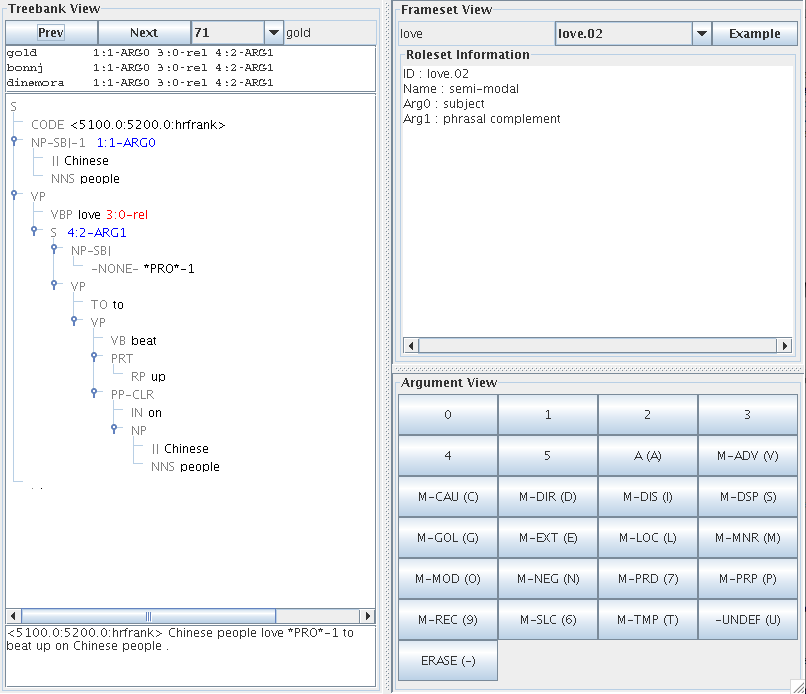
\includegraphics[scale=0.4]{img/SComplement.png}
\caption{\texttt{S} as sentential complement}
\label{fig: SComplement}
\end{figure}

As mentioned previously, the \texttt{rel} can potentially arise in other types of nodes, such as \texttt{NP} (noun phrase) or \texttt{ADJP} (adjective phrase) nodes, with or without an intervening \texttt{VP} node.  When this happens, the annotation span cannot be thought of as delimited by an \texttt{S} node.  Just as in previously mentioned cases, annotate sisters to the verb or \texttt{VB} TreeBank tag and annotate sisters to the \texttt{VP} node when present.  Although the \texttt{S} node will not be present as a clue for where to stop annotation, simply do not annotate constituents that are parents or aunts to the verb or verb phrase node.  Parents and aunts, unlike sisters, will not be along a parallel line with the verb or verb phrase.  Instead, their root nodes will be located to the left of this line.  This heuristic applies when determining the span of any annotation, but may be especially important in the absence of an \texttt{S} node.  

Figure~\ref{fig: NPRel} gives an example of a \texttt{rel} contained within an \texttt{NP} node.  Note that the \texttt{NP} node itself and everything outside of this node should not be annotated because these constituents are parents or aunts of the verb phrase rather than sisters of the verb phrase or verb. 

\begin{figure}[htbp]
\centering
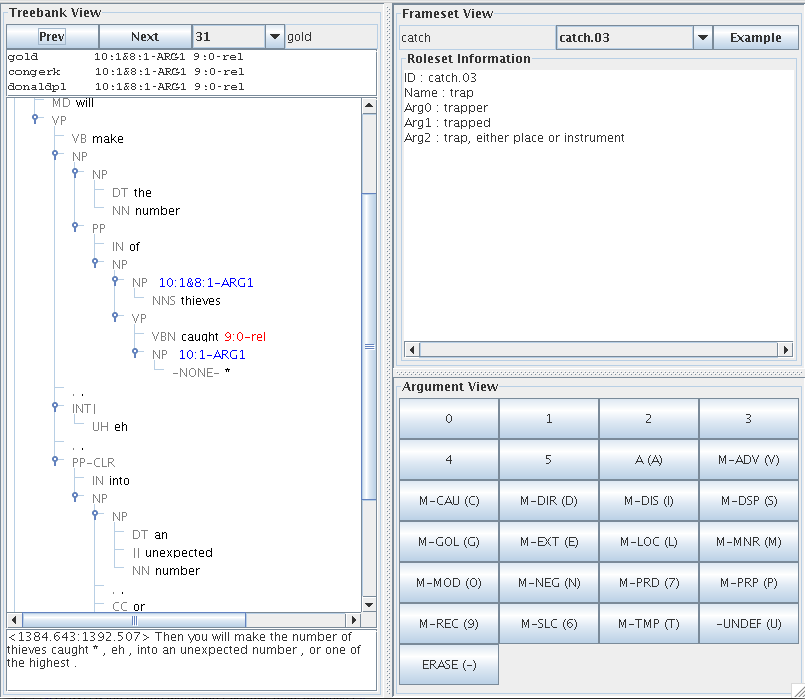
\includegraphics[scale=0.4]{img/NPRel.png}
\caption{\texttt{rel} embedded in an \texttt{NP} node}
\label{fig: NPRel}
\end{figure}

\section{Where to Place Tags}
Jubilee allows you to select any node in the tree; thus, it is up to the annotator to select the appropriate node reflecting the correct constituent boundaries of an argument.  In general, the node above the lexical item itself, which indicates the syntactic function of that constituent (e.g., \texttt{NP}, \texttt{NP-SBJ}, \texttt{PP}, \texttt{ADJP}, \texttt{ADVP}, etc.), is the correct placement for the tag.  However, as mentioned in the ARGM sections, annotation of modals and negatives require placement of the tag directly on the lexical item because there is no higher node to annotate without including more than just the modal or negative marker.  Please review the Jubilee screen shots given in Section~\ref{sec: span} for examples of the correct placement of tags.  

Occasionally, the phrase structure of an instance is such that the annotator must choose between annotating a higher node as a single argument or annotating several nodes embedded therein as various arguments.  As a general rule of thumb, if it is possible to place a lower-numbered argument tag on a single, higher node, this is preferable to annotating several higher-numbered arguments and/or modifiers on embedded nodes therein.  For example, Figure~\ref{fig: BadArgPlacement} below is correct given the argument structure outlined in the frame \texttt{hold.04}, but it is dispreferred to Figure~\ref{fig: ArgPlacement}, which simply tags the higher node with a lower argument number.

\begin{figure}[htbp]
\centering
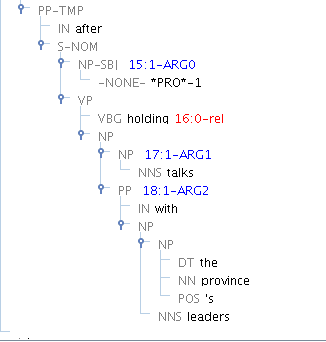
\includegraphics[scale=0.4]{img/BadArgPlacement.png}
\caption{Theoretically correct, but dispreferred annotation}
\label{fig: BadArgPlacement}
\end{figure}

\begin{figure}[htbp]
\centering
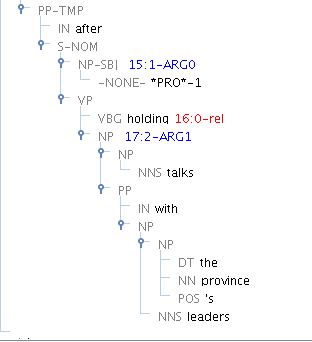
\includegraphics[scale=0.4]{img/ArgPlacement.png}
\caption{Preferred annotation of higher node with lower argument number}
\label{fig: ArgPlacement}
\end{figure}

\subsection{Exceptions to Normal Tag Placement}
Certain verbs such as \textit{encourage} and \textit{persuade}, which involve both an impelled agent and an impelled action require that annotators \textit{break up} and delve into the sister \texttt{S} node in order to annotate the impelled agent and impelled action separately.  These are often cases of verbs that participate in exceptional case marking, meaning that the matrix verb (e.g., \textit{encourage} or \textit{persuade}) assigns the accusative case to the subject of the sentential complement: 

\textit{I encouraged \textbf{him} to annotate for PropBank.} \\
\**\textit{I encouraged \textbf{he} to annotate for Propbank.} 

Because the matrix verb assigns accusative case to the subject of the infinitival complement,  it is thought that the verb assigns semantic roles to both the agent and action separately.  In some cases, such usages are parsed with two separate constituents that can be marked as usual with separate arguments: an \texttt{NP} node for the impelled agent and an \texttt{S} node for the action.  However, in  other cases, the sentential complement of these verbs forms a single constituent, which is an \texttt{S} node that is a sister to the matrix verb.  As a result, where we would normally only annotate the \texttt{S} node with an argument, in these cases, we annotate within the \texttt{S} node to separately tag the impelled agent and impelled action.  These are essentially theoretical disagreements in how to parse such instances.  As always, annotators should allow the rolesets to guide their annotations.  

\section{Understanding and Annotating Null Elements in the Penn TreeBank}
\label{sec: null1}
The inventory of null elements used in Penn TreeBank is as follows: 

\begin{tabular}{ll}
	\texttt{[*PRO*]} & overt subjects, subject control, and small clauses \\ \relax
	\texttt{[*]} & passive traces including reduced relative clauses and raising constructions \\ \relax
	\texttt{[*T*]} & trace of A-movement, including parasitic gaps \\ \relax
	\texttt{[(NP *)]} & arbitrary PRO, controlled PRO, and trace of A-movement  \\ \relax
	\texttt{[0]} & null complementizer, including null wh-operator \\ \relax
	\texttt{[*U*]} & unit \\ \relax
	\texttt{[*?*]} & placeholder for ellipsed material \\ \relax
	\texttt{[*NOT*]} & anti-placeholder in template gapping \\ \relax
	\texttt{[*RNR*]} & pseudo-attach: right node raising \\ \relax
	\texttt{[*ICH*]} & pseudo-attach: interpret constituent here \\ \relax
	\texttt{[*EXP*]} & pseudo-attach: extraposition \\
\end{tabular}

This section presents some examples of most commonly used null elements and their PropBank annotation.

\subsection{Passive Sentences} 

Sentences can be either active (`\textit{The executive committee approved the new policy}') or passive (`\textit{The new policy was approved by the executive committee}'). In active sentences, the subject is the agent or do-er of the action, marked as ARG0 in PropBank. In passive sentences, the subject of the sentence is acted upon by some other agent or by something unnamed, and is being marked as ARG1 in PropBank. 

Passive sentences are assumed to be derived from the corresponding active sentences by movement of the object to the subject position. This movement leaves a trace, represented as \texttt{[*]} in TreeBank.  Except in the case of reduced relatives, this trace will already be coindexed with its realized referent: 
                        
Active: \textit{Mary hit John} \\
Passive: \textit{John-1 was hit [*-1] by Mary.}

Since TreeBank provides a link between \texttt{[*-1]} and \textit{John},  it is the trace, rather than the \texttt{NP} \textit{John}, which is being labeled as ARG1 in PropBank: 

\textit{PropBank annotation:}\\
REL:            hit\\
ARG1:        	[*-1]\\
ARG0:           by Mary

The following example illustrates a TreeBank representation of the passive sentence. The link between the trace and the \texttt{NP} is indicated by the number 1 in the trace \texttt{(NP-3 *-1)} and \texttt{(NP-SBJ-1 he)} below.  Note that chains of coreference are represented in the Penn TreeBank using various numerals, and that one element such as `he' can potentially be semantically present in several positions in the underlying syntax; therefore, several numbered indices may be connected to one element.  It is important to follow the chains of coreference throughout the instance to ensure a full understanding of each null element.  

\textit{TreeBank annotation:}
\begin{verbatim}
  (S (NP-SBJ-1 he)
     (VP was
         (VP accused
             (NP-3 *-1)
             (PP-CLR of
                     (S-NOM (NP-SBJ *-3)
                            (VP (VP conducting
                                    (NP illegal business))
                                and
                                (VP possessing
                                    (NP illegal materials))))))))
\end{verbatim}

Again, it is the trace which is being annotated as the argument:

\textit{PropBank annotation:}\\
ARG1: [NP-3 *-1] \\
REL: accused\\
ARG2: of [*3*] conducting illegal business and possessing illegal materials

\subsection{Fronted and Dislocated Arguments}

Other examples of moved constituents are fronted or otherwise dislocated arguments and adjuncts. As in the other cases of movement, fronted elements leave a trace, which is being coindexed with the moved constituent in TreeBank. 

In the following example, the ARG2 (`\textit{where put}') argument of the verb \textit{put} is being fronted. In the TreeBank annotation, this is indicated by the chain which links the trace \texttt{[*T*-1]} with the adverbial \textit{There}:

\textit{TreeBank annotation:}
\begin{verbatim}
  (S (ADVP-PUT-TPC-1 There)
     ,
     (NP-SBJ I)
     (VP put
         (NP the book)
         (ADVP-PUT *T*-1) ))
\end{verbatim}

As with annotation of passive traces, the ARG2 argument is the trace, rather than the fronted constituent:

\textit{PropBank annotation:}
REL:	put\\
ARG0:	I\\
ARG1:	the book\\
ARG2:	[*T*-1] 

Modifiers, or ARGMs, can be fronted as well, as the following example shows:

\textit{TreeBank annotation:}
\begin{verbatim}
(S (SBAR-PRP-TPC-9 Because
                     (S (NP-SBJ I)
                        (VP 'm
                            (NP-PRD such a bad boy))))
     (NP-SBJ I)
     (VP think
         (SBAR 0
               (S (NP-SBJ I)
                  (VP wo n't
                      (VP get
                          (NP a lollipop)
                          (SBAR-PRP *T*-9) )))))
\end{verbatim}
Since the `\textit{because}' clause modifies the verb \textit{get} in this example, the trace originates as the modifier of \textit{get}. This trace is being annotated as ARGM-CAU in PropBank:

\textit{PropBank annotation:}\\
REL:		get\\
ARG1:		a lollipop\\
ARG0:		I\\
ARGM-NEG:	n't\\
ARGM-MOD:	wo\\
ARGM-CAU:	[*T*-9]

In rare situations, movement does not leave a trace, but rather leaves a pronoun (called a resumptive pronoun). In such cases, the argument of the verb is a higher \texttt{NP}, which includes both the pronoun and the trace to the topicalized \texttt{NP} in TreeBank. This \texttt{NP} is annotated as ARG1 in PropBank:

\textit{TreeBank annotation:}
\begin{verbatim}
  (S (NP-TPC-1 John)
     ,
     (NP-SBJ I)
     (VP like
         (NP (NP him)
	             (NP-1 *T*))
         (NP-ADV a lot)))
\end{verbatim}

\textit{PropBank annotation:}\\
REL:	like\\
ARG0:	I\\
ARG1:	[NP (NP him) (NP-1 *T*)]\\
ARGM-MNR:	a lot

In even more rare situations, the topicalized \texttt{NP} and the pronoun are not already co-indexed in the TreeBank. See Section~\ref{sec: specialTopicalization} for further description of how to annotate these instances. 

\subsection{Questions and Wh-Phrases}

Another type of traces is a trace of a wh-phrase in questions.

\textit{What do you like?}

As in the case of passive sentences, questions are assumed to be derived by movement.  In the example below, the ARG1 argument of the verb \textit{like} is a wh-phrase \textit{what}, which moves from the object position of the verb to the front of the sentence. This movement leaves a trace, as shown below:

\textit{What-1 do you like [*T*-1]?}

In TreeBank annotations, wh-phrases are marked as WHNP. As in the case of passive sentences, TreeBank provides a link between the trace and the moved WHNP:

\textit{TreeBank annotation:}
\begin{verbatim}
  (SBARQ (WHNP-1 what)
         (SQ do
             (NP-SBJ you)
             (VP like
                  (NP *T*-1)))
\end{verbatim}

Again, for the purposes of PropBank, the argument ARG1 is the trace, as shown below:

\textit{PropBank annotation:}\\
REL: like\\
ARG0: you\\
ARG1: [*T*-1]

Wh-phrases are not necessarily core arguments. However, questions can be formed with wh-phrases like \textit{when}, \textit{where}, or \textit{how}, in which case they should be tagged as ARGMs.  

\textit{TreeBank annotation:}
\begin{verbatim}
SBARQ (WHNP-1 Which day)
         (SQ did
             (NP-SBJ you)
             (VP get
                 (ADVP-DIR there)
                 (NP-TMP *T*-1)))
\end{verbatim}

\textit{PropBank annotation:}\\
ARG0:           	you\\
REL:            	get\\
ARG2: there\\
ARGM-TMP:       [*T*-1] 

\textit{TreeBank annotation:}
\begin{verbatim}
  (SBARQ (WHADVP-42 How)
         (SQ did
             (NP-SBJ you)
             (VP fix
                 (NP the car)
                 (ADVP-MNR *T*-42)))
         ?)
\end{verbatim}

\textit{PropBank annotation:}\\
REL: fix\\
ARG0: you\\
ARG1: the car\\
ARGM-MNR:  [*T*-42]

Questions can also be embedded, as in the example below. PropBank annotation is not different from direct questions in this case:

 \textit{John didn't know where-3 his parents had met [*T*-3].}

ARG0:          	 his parents    \\           
REL:           	 met\\
ARGM-LOC:       [*T*-3]
 
\subsection{Interpret Constituent Here (ICH) Traces}
  
\texttt{ICH} traces are used in TreeBank to indicate a relationship of constituency between elements separated by intervening material. An example of such split constituents are `heavy shift' constructions, illustrated below:

\textit{TreeBank annotation:}
 \begin{verbatim}
  (S (NP-SBJ (NP a young woman)
             (SBAR *ICH*-1))
     (VP entered
         (SBAR-1 (WHNP-2 whom)
                 (S (NP-SBJ she)
                    (PP-TMP at
                            (ADVP once))
                    (VP recognized
                        (NP *T*-2)
                        (PP-CLR as
                                (NP Jemima Broadwood)))))))
 \end{verbatim}

The subject \texttt{NP} in this case is being split into two constituents: the \texttt{NP} `\textit{a young woman}' and \texttt{SBAR} `\textit{whom she at once recognized as Jemima Broadwood}.' The \texttt{ICH} trace specifies a link to the \texttt{SBAR} node in this example.  Essentially, the \texttt{NP} in addition to the material linked by \texttt{ICH} trace can be thought of as one whole constituent: `\textit{A young woman whom she at once recognized as Jemima Broadwood},' part of which has been moved for pragmatic purposes. 

In all examples of this type, the argument is the constituent which includes the \texttt{ICH} trace:  

\textit{PropBank annotation:}\\
ARG0: a young woman [ICH-1]\\
REL:  entered
 
 It is very important that the annotator does not annotate the dislocated part of the constituent (in the previous case the \texttt{SBAR-1} material) a second time with another tag.  Underlyingly, the material connected by \texttt{ICH} trace is part of the \texttt{NP} `\textit{a young woman},' which is already annotated as ARG0.  In post-processing, the rest of this constituent linked by \texttt{ICH} trace will be concatenated to the \texttt{NP} annotated as ARG0; thus, tagging the dislocated portion of the constituent a second time will create recursive annotation and will be returned as an error.  In other words, tagging the dislocated portion will be recognized computationally as having a second argument of a different type embedded in the first, which is disallowed.  

Other typical examples of \texttt{ICH} traces are shown below:

\textit{[Five ICH-1] ran, [out of the twenty-five that showed up]-1.}\\
ARG0:        Five *ICH-1*\\
REL:            ran

\textit{[Some people in Paris]-1 want *PRO*-1 to hear more [ICH-2] from me [than those fellers over at the conference house do]-2.}\\
ARG0: *PRO*-1\\
REL:	hear\\
ARG1:  more [ICH-2]\\
ARG2:  from me
	
Figure~\ref{fig: ICH} shows correct annotation for an instance containing an \texttt{ICH} trace.  

\begin{figure}[htbp]
\centering
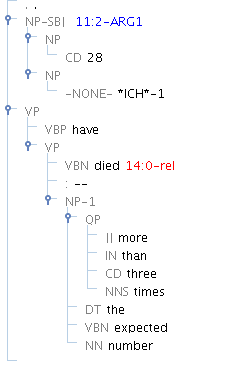
\includegraphics[scale=0.6]{img/ICH.png}
\caption{Correct annotation of \texttt{ICH}}
\label{fig: ICH}
\end{figure}

\subsection{Right Node Raising (RNR) Traces}

\texttt{RNR} traces are used when a constituent is interpreted simultaneously in more than one place. An example of a right node raising structure is given below:

\textit{TreeBank annotation:}
 \begin{verbatim}
(NP (NP (ADJP so many) enchained demons)
      (VP straining
          (PP-MNR in
                  (NP anger))
          (S (NP-SBJ *)
             (VP to
                 (VP (VP tear
                         (NP *RNR*-1))
                     and
                     (VP gnaw
                         (PP-CLR on
                                 (NP *RNR*-1)))
                     (NP-1 his bones))))))
 \end{verbatim}

In this example, the \texttt{NP} `\textit{his bones}' is interpreted as both the argument of the verb \textit{tear} and the verb \textit{gnaw}. When annotating the verb \textit{tear}, the trace, \texttt{(NP *RNR*-1)}, is the argument of the verb:

\textit{PropBank annotation:}\\
REL: tear\\
ARG1: [*RNR*-1]\\ 
ARG0: [NP-SBJ*] 

Likewise, when annotating the verb \textit{gnaw}, the prepositional phrase, including the trace \texttt{(PP-CLR on (NP *RNR*-1)))}, is analyzed as the argument:

\textit{PropBank annotation:}\\
REL:  gnaw\\
ARG1: on [*RNR*-1]\\ 
ARG0: [NP-SBJ*] 

A similar annotation applies when the \texttt{RNR} trace is a clausal argument:

\textit{I want *RNR*-1 and like *RNR*-1 [* to eat ice-cream]-1.}\\
ARG0:           I\\
REL:            want\\
ARG1:           *RNR*-1

If the \texttt{RNR} trace is part of the argument of the verb, then select the argument including the trace:

\textit{His dreams had revolved around her so much and for so long that...}

\textit{TreeBank annotation:}
 \begin{verbatim}
  (S (NP-SBJ His dreams)
     (VP had
         (VP revolved
             (PP-CLR around
                     (NP her))
             (UCP-ADV (ADVP (ADVP so much)
                            (SBAR *RNR*-1))
                      and
                      (PP-TMP for
                              (NP (NP so long)
                                  (SBAR *RNR*-1)))
                      (SBAR-1 that...)))))
\end{verbatim}
 
\textit{PropBank annotation:}\\
ARG1:	his dreams\\
REL: 	revolved\\
ARGM-LOC: around her\\
ARGM-EXT:  so much [*RNR*] 

The following example illustrates annotation of \texttt{RNR} traces within a small clause (for further information on the annotation of small clauses, see Section~\ref{sec: smallClauses}). 

\textit{But our outlook has been and continues to be defensive}
 
\textit{TreeBank annotation:}
 \begin{verbatim}
  (S But
     (NP-SBJ-2 our outlook)
     (VP (VP has
             (VP been
                 (ADJP-PRD *RNR*-1)))
         ,
         and
         (VP continues
             (S (NP-SBJ *-2)
                (VP to
                    (VP be
                        (ADJP-PRD *RNR*-1)))))
         ,
         (ADJP-PRD-1 defensive)))
\end{verbatim}
 
\textit{PropBank annotation:}\\
REL:   continue\\
ARG1: [*-2] to be *RNR-1

Figure~\ref{fig: RNR} shows correct annotation of an instance containing \texttt{RNR} traces. 

\begin{figure}[htbp]
\centering
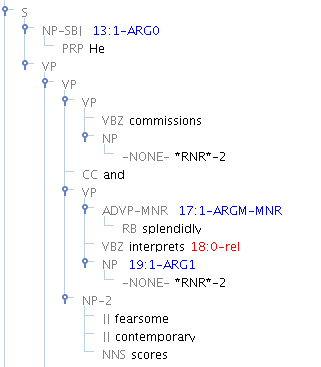
\includegraphics[scale=0.6]{img/RNR.png}
\caption{Correct annotation of \texttt{RNR}}
\label{fig: RNR}
\end{figure}

\subsection{It EXtraPosition (EXP)}

Dummy placeholders in English such as \textit{it} or \textit{that} do not add any meaning to the sentence.  In the following example, the syntactic subject of the sentence is a dummy \textit{it}, which includes a trace \texttt{*EXP*-1}. This trace refers to the logical, semantic subject of the sentence, marked as \texttt{SBAR-1}:

\textit{TreeBank annotation:}
 \begin{verbatim}
  (S (NP-SBJ (NP It)
             (SBAR *EXP*-1))
     (VP is
         (ADJP-PRD clear)
         (PP to
             (NP me))
         (SBAR-1 that
                 (S (NP-SBJ this message)
                    (VP is
                        (ADJP-PRD unclear))))))
\end{verbatim}
 
In PropBank annotations, dummy \textit{it} and \texttt{EXP} traces are \textbf{not included, do not tag them}:

\textit{PropBank annotation:}\\
REL: is\\
ARG1: that this message is unclear\\
ARG2: clear to me

Rather, tag only that which has semantic value in the utterance, the overt constituent.  Thus, the underlying phrase can be thought of semantically as: `\textit{That this message is unclear is clear to me}.'  The \textit{it} is merely added for pragmatic purposes to avoid having such a heavy constituent at the front of the phrase.  
 
 Another example:

\textit{It required an energy he no longer possessed to be satirical about his father.}

\textit{PropBank annotation:}\\
ARG0: to be satirical about his father\\
ARG1: an energy he no longer possessed\\
REL: required

In the examples below, the dummy constituents are the objects, rather than the subjects. As in the case of dummy subjects, only the logical argument is being tagged, whereas the dummy pronoun and the \texttt{EXP} trace are not part of the PropBank annotation:

\textit{Mrs. Yeargin was fired [*-1] and prosecuted [*-1] under an unusual South Carolina law that-79 [*T*-79] makes it [*EXP*-2] a crime [*] to breach test security.}

\textit{PropBank annotation:}\\
ARG0:       [*T*-79] \\
REL:        makes\\
ARG2:   a crime\\
ARG1:   [*] to breach test security

\textit{Any raider would find it [*EXP*-1] hard [*] to crack AG 's battlements.}

\textit{TreeBank annotation:}
 \begin{verbatim}
(S 
    (NP-SBJ (DT Any) (NN raider) )
    (VP (MD would) 
      (VP (VB find) 
        (S 
          (NP-SBJ 
            (NP (PRP it) )
            (S (-NONE- *EXP*-1) ))
          (ADJP-PRD (JJ hard) )
          (S-1 
            (NP-SBJ (-NONE- *) )
            (VP (TO to) 
              (VP (VB crack) 
                (NP 
                  (NP (NNP AG) (POS 's) )
                  (NNS battlements) )))))))
    (. .) )
 \end{verbatim}

\textit{PropBank annotation:}\\
ARG0:       Any raider\\
ARGM-MOD:   would\\
REL:        	find\\
ARG3:      	 hard\\
ARG1:	     	[*] to crack AG 's battlements\

Figure~\ref{fig: EXP} shows correct annotation of an instance of the copular sense of \textit{to be}, which contains it \texttt{EXP}. 

\begin{figure}[htbp]
\centering
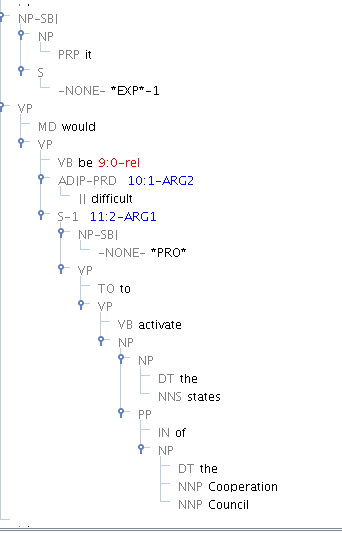
\includegraphics[scale=0.6]{img/itexp.png}
\caption{Correct annotation of \texttt{EXP} and \texttt{be.01}}
\label{fig: EXP}
\end{figure}

Common mistake: Please make sure to distinguish dummy \textit{it} from the referring pronoun \textit{it}, where \textit{it} refers to a previous \texttt{NP}, a clause, or an event. (hint: referring pronouns are not followed by an \texttt{EXP} trace in TreeBank). All referring pronouns, including \textit{it}, should be marked as arguments in PropBank.

\textit{It sounds good.}\\
REL: 	sounds\\
ARG1:	 it\\
ARGM-MNR: 	good

\textit{Italy's Foreign Ministry said [0] it is investigating exports to the Soviet Union.}\\
REL: investigating\\
ARG0: it\\
ARG1: exports to the Soviet Union

\subsection{Other Traces}

Other types of traces include the null complementizer trace, \texttt{0}, the \texttt{?} trace (used in ellipsis constructions), and the \texttt{PPA} trace in cases of predictable ambiguous attachments. 

Null complementizer traces should be included as part of the clausal argument; thus, the ARG1 in this case would be annotated at the level of the \texttt{SBAR} node:

\textit{TreeBank annotation:}
 \begin{verbatim}
 (S (NP-SBJ I)
     (VP believe
         (SBAR 0
               (S (NP-SBJ you)
                  (VP are
                      (ADJP-PRD smart))))))
\end{verbatim}
 
\textit{PropBank annotation:}\\
REL: believe\\
ARG0: I\\
ARG1: [[0] you are smart]

\section{Linking and Annotation of Null Elements}
\label{sec: null2}
\subsection{SeLectional Constraint Link (Link SLC)}
\label{ssec: SLC}
\subsubsection{Relative Clause Annotation}

\paragraph{Typical Relative Clauses}
Relative clauses are clauses that modify an \texttt{N} or an \texttt{NP} as in `\textit{answers that we'd like to have.}'  Relative clauses also include a trace, which is coindexed with the relativizer in TreeBank (e.g., \textit{that}, \textit{which}, \textit{who}).  Alternatively, the relativizer can be omitted in English: `\textit{answers we'd like to have.}'  In these cases the TreeBank will still include a placeholder for the relativizer, but a \texttt{0} will appear where the explicit relativizer normally appears.

\noindent For example, in the following TreeBank annotation, the object position of the verb has a trace \texttt{(NP *T*-6)}, which is being coindexed with the relativizer \texttt{(WHNP-6 that/which/0)}. 

\textit{TreeBank annotation:}
\begin{verbatim}
  (NP (NP answers)
       (SBAR (WHNP-6 that/which/0)}
            (S (NP-SBJ-3 we)
               (VP 'd
                   (VP like
                       (S (NP-SBJ *-3)
                          (VP to
                              (VP have
                                  (NP *T*-6)))))))))
\end{verbatim}                                  

Whereas, syntactically, the trace is being coindexed with the relativizer,  semantically, there is a relationship between the trace and the \texttt{NP} \textit{answers}, which is not being represented in TreeBank. This relationship is now captured via post-processing, so annotators do not need to provide any link here, but should be aware of how to recognize and understand the relationships between elements in a relative clause structure. 

\subsection{Pragmatic Coreference Link (Link-PCR)}
Link-PCR is annotated through the use of the \texttt{*}  function in Jubilee.  Later, in post-processing, this function is converted to the Link-PCR label.  Reduced relative links are captured strictly via post-processing, but are also converted to the same type of link. 

\subsubsection{Reduced Relative Annotation}

A relative clause may be reduced when passive, resulting in the unique syntax of a reduced relative clause.  For example, a passive relative clause construction such as `\textit{\textbf{The woman that was dressed in blue} walked past the house}' can be reduced to `\textit{\textbf{The woman dressed in blue} walked past the house.}'  Because the verb in these cases is always passive, the TreeBank annotation of reduced relatives will include an object trace after the verb.  However, unlike normal passive constructions, this trace will never be coindexed with the subject.  The annotator can simply tag the trace as an ARG1 and rely on post-processing to capture the relationship between the trace and the subject. Figure~\ref{fig: redrelex} shows a reduced relative construction that annotators are able to link. 

\textit{TreeBank Annotation:}
\begin{verbatim}
(S
  (NP-SBJ-1
    (DT This)
  (VP
    (VBZ is)
    (VP
      (VBN considered)
      (S
        (NP-SBJ
          (-NONE- *-1)
        (NP-PRD
          (NP
            (CD one)
          (PP
            (IN of)
            (NP
              (NP
                (DT the)
                (JJS biggest)
                (NNS caches)
              (VP
                (VBN seized)
                (NP
                  (-NONE- *)
                (PP-LOC
                  (IN in)
                  (NP
                    (DT the)
                    (NN district)
\end{verbatim}
                    
\textit{PropBank Annotation:}\\
REL: seized\\
ARG1: [NP -NONE- *] \\
ARGM-LOC: [PP-LOC in the district]

\begin{figure}[htbp]
\centering
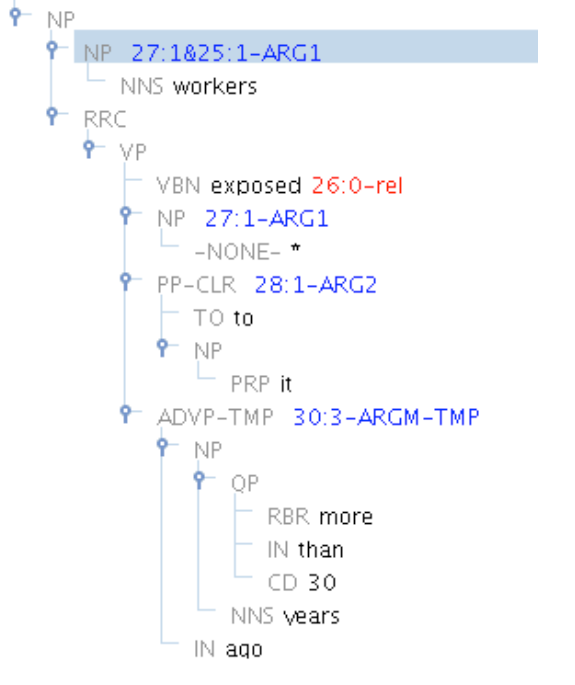
\includegraphics[scale=0.4]{img/redrelex.png}
\caption{Example of a Reduced Relative annotation}
\label{fig: redrelex}
\end{figure}

\subsubsection{Annotation of PRO}
\label{sec: PRO}

Many traces found in the TreeBank arise as a result of the movement of a constituent from its canonical position.  Movement leaves a trace, represented by a \texttt{*} or a \texttt{*T*} in the TreeBank.  \texttt{PRO}, on the other hand, does not arise as a result of movement.  Rather, \texttt{PRO} arises where there is an underspecified, or unrealized subject of a verb.  For example, the subject of the verb \textit{leave} in the phrase `\textit{she tried to leave}' is not realized.  However, the TreeBank will represent the unrealized subject of \textit{leave} with \texttt{PRO}: 

\textit{She-1 tried *PRO*-1 to leave}\\
REL: leave\\
ARG0: *PRO*-1

In cases like that of the example above, the \texttt{PRO} element is already coindexed with the fully realized subject because the \texttt{PRO} is positioned in a clause that is governed by the higher clause with the same subject, \textit{she}.  Thus, the annotator need not add any additional links between \texttt{PRO} and the explicit subject.  However, there are also cases in which \texttt{PRO} arises but it is not governed by a higher clause.  In these cases, it is not coindexed with a fully realized subject.  Figure~\ref{fig: Nonrefitpro} shows an example of a \texttt{PRO} which has no referent in this sentence. 

When annotating \texttt{PRO} that is not indexed, if the annotator is certain that the subject is realized elsewhere in the instance, then a link should be created between \texttt{PRO} and the explicit reference. If the annotator is \textbf{not absolutely certain} that the explicit reference and \texttt{PRO} share the same referent, then the annotator should not create the link.  Essentially, unless the relation is absolutely certain, we should err on the side of agreeing with the TreeBank annotation and its existing indices. In the cases where the annotator has decided with certainty that a link should be created between the \texttt{PRO} argument and a fully realized subject: first, annotate \texttt{PRO} with its appropriate argument, then select the node of the explicit subject mention associated with \texttt{PRO}, and finally, click {\tt Argument} on the Jubilee menu bar, followed by clicking {\tt Functions}.  From the options therein, select \texttt{*} (shortcut: \texttt{Ctrl+Shift+8}).  At this point, the linked annotation should appear on the currently selected node of the explicit referent.  An example of this is also given in Figure~\ref{fig: PROann}.

\begin{figure}[htbp]
\centering
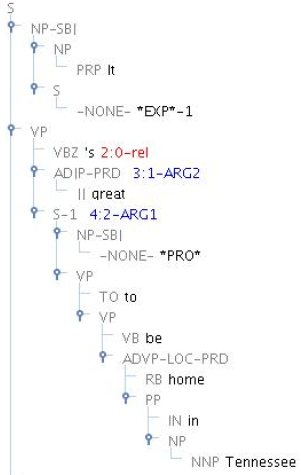
\includegraphics[scale=0.5]{img/Nonrefitpro.png}
\caption{Example of a nonreferential \textit{it} \texttt{PRO}}
\label{fig: Nonrefitpro}
\end{figure}
\begin{figure}[htbp]
\centering
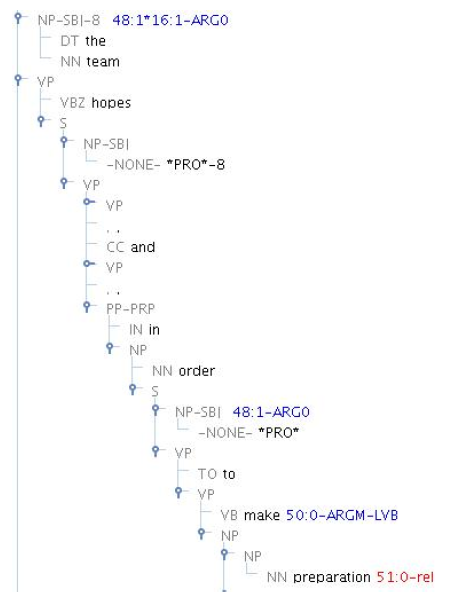
\includegraphics[scale=0.5]{img/PROann.png}
\caption{Example of \texttt{PRO} annotation}
\label{fig: PROann}
\end{figure}

The goal of this annotation is to provide additional semantic information about the arguments of the verbs.  In some cases, antecedents are not syntactic constituents, or have a different morphological form, as the possessive pronoun \textit{your} below illustrates; forego linking in these cases:

\textit{On the issue of abortion , Marshall Coleman wants  to take away your right  [*] to choose and give it to the politicians.}\\
ARG0:          [*PRO*]\\
REL:           choose

Additionally, note that the null element should be linked to the highest possible node containing its referent without recursively annotating other arguments or the \texttt{rel} itself (i.e. creating arguments embedded within other arguments).  If this is not possible, the link should be omitted. 

\subsection{Concatenation of multiple nodes into one argument}
\label{sec: concatenation}
As a rule, annotations should be placed on the highest node possible encompassing the entirety of a constituent (e.g., the \texttt{NP} or \texttt{PP} level in the TreeBank), and one tag should correspond to one node for every node within the appropriate annotation span.  However, in some cases the \texttt{rel} is situated within an \texttt{NP} node, and the manner in which the TreeBank is laid out makes it impossible to capture a whole constituent under one node.  In these cases, two leaves of the tree may have to be concatenated together under a single argument label.  Figure~\ref{fig: concatarg} shows an example of this. 

\begin{figure}[htbp]
\centering
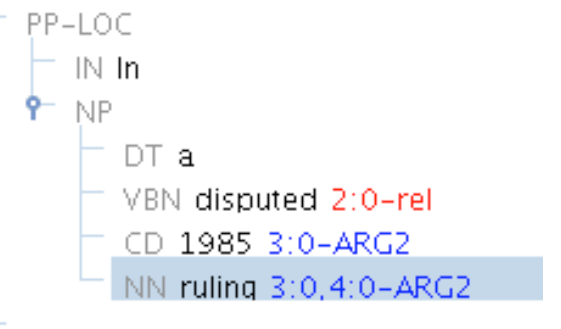
\includegraphics[scale=0.3]{img/concatarg.png}
\caption{Example of a Concatenated Argument}
\label{fig: concatarg}
\end{figure}

To concatenate two leaves into a single argument, first select the node of the first word of the constituent (e.g. \textit{1985}) and then click the appropriate button (e.g, \texttt{2}) indicating which semantic role the argument is playing.  Next, select the node of the second word of the constituent (e.g. \textit{ruling}) and navigate to {\tt Argument} on the Jubilee menu bar, followed by clicking {\tt Functions}.  From the options therein, select \texttt{,} (shortcut: \texttt{Ctrl+Shift+,}). The resulting annotation will reflect the tree location of both nodes as part of a single argument (e.g. {\tt 3:0,4:0-ARG1}).

In cases of passive extraction of the subject and subject raising verbs like \textit{seem}, concatenation can also be required to put the subject and clause following the verb under one argument label.  See Section~\ref{sec: smallClauses} for more discussion of this topic.  

Another instance of concatenation involves verb particle constructions, such as \textit{stalled out} in Figure~\ref{fig: PRTconcat}. Many of these verbs will have a frame set especially for particle instances.

\begin{figure}[htbp]
\centering
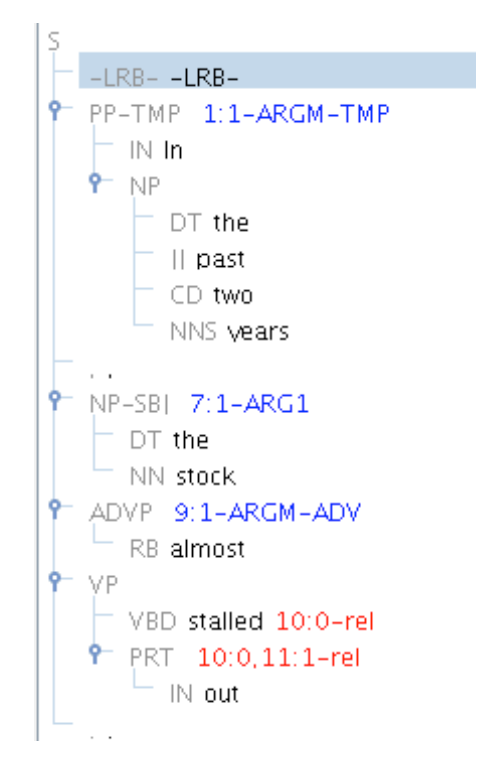
\includegraphics[scale=0.4]{img/PRTconcat.png}
\caption{Example of a verb particle in Jubilee}
\label{fig: PRTconcat}
\end{figure}

\subsection{Special cases of topicalization}
\label{sec: specialTopicalization}
Topicalization occurs when a constituent is moved from its underlying syntactic position to an atypical position in order to draw attention to that constituent.  Although the majority of cases of topicalization simply require annotation of a trace that is already indexed to the topicalized constituent, occasionally the topicalized constituent is repeated, often in the form of a pronoun, and the two constituents are not already indexed in the tree.  For example, `\textit{911, that's the number you call in an emergency.}'  If the \texttt{rel} to be annotated is \textit{is}, the annotator would firstly have to annotate the pronoun \textit{that} as ARG1, then provide a coreference link to the pronoun's referent, \textit{911}.  Performing this link works in an identical manner to that of creating coreference links for \texttt{PRO} seen in Section~\ref{sec: PRO}.  Thus, after selecting and annotating the pronoun in the argumental position, subsequently select the topicalized node and click {\tt Argument} on the Jubilee menu bar, followed by clicking {\tt Functions}.  From the options therein, select \texttt{*} (shortcut: \texttt{Ctrl+Shift+8}).  The linked annotation should appear in the TreeBank view and in the annotation view at the top of the screen.  For example: 

\textit{TreeBank Annotation:}
\begin{verbatim}
(S
  (NP-SBJ
    (PRP I))
  (VP
    (VBD expected)
    (NP
      (PRP it))
    (PP-LOC
      (IN in)
      (NP
        (NP
          (DT a)
          (NN country))
        (SBAR
          (WHNP-1
            (-NONE- 0))
          (S
            (NP-SBJ
              (PRP we))
            (VP
              (VBP love)
              (NP
                (-NONE- *T*-1))
              (, ,)
              (NP-TPC
                (PRP me)
                (CC and)
                (PRP you))))))))
\end{verbatim}

\textit{PropBank annotation:}\\
REL: love\\
ARG1: (NP (-NONE- *T*-1))\\
ARG0: [NP-SBJ we] *[NP-TPC me and you]

 \section{Special Cases: small clauses and sentential complements}
 \label{sec: smallClauses}
This section is concerned with different types of clausal complements and modifiers, with a special focus on passive extraction, subject-raising verbs, and aspectual verbs. 
In the following sentence, the clause \texttt{S-CLR} has a trace in the subject position of \textit{asleep}, which is coindexed with the subject of the verb \textit{fell}, \textit{I}. 

\textit{I fell asleep on the floor.}
 
\textit{TreeBank annotation:}
 \begin{verbatim}
S (NP-SBJ-1 I)
     (VP fell
         (S-CLR (NP-SBJ *-1)
                (ADJP-PRD asleep))
         (PP-LOC on
                 (NP the lobby floor))))
 \end{verbatim}

When annotating the verb \textit{fell}, the small clause (marked as \texttt{S-CLR} above) is tagged as ARGM-PRD, and the ARG1 argument is the \texttt{NP-SBJ} \textit{I}. Note that although the empty category \texttt{NP-SBJ *-1} is being coindexed with \textit{I}, the trace is not the argument of \textit{fell}, but rather is the subject of \textit{asleep}. 

\textit{PropBank annotation:}\\
REL:	fell\\
ARG1:	I\\
ARGM-PRD: [NP-SBJ *-1] asleep

Verbs like \textit{expect} are analyzed as having a clause as its argument (which corresponds to the event expected). In this case PropBank annotation follows TreeBank analysis of these sentences, where the clausal complement is being selected as ARG1:

\textit{John expected Mary to come.}

\textit{PropBank Annotation}\\
REL: 	expected\\
ARG0:	John\\
ARG1:	Mary to come

If such sentences are passivised, as shown below, then the ARG1 argument is the clausal complement of the verb. Parallel to \texttt{ICH} and \texttt{RNR} traces, we assume that the trace \texttt{[*-1]} is being `reconstructed,' so that the ARG1 in this case corresponds to the proposition `\textit{Mary to come}'. It is necessary to annotate the dislocated portion (e.g. \texttt{NP Mary-1}) as part of the ARG1 via concatenation using the \texttt{,} operator, discussed in Section~\ref{sec: concatenation}.  The process by which the subject is raised from the clausal complement to become the subject of the matrix verb, \textit{expect}, is sometimes called passive extraction. 

\textit{Mary-1 is expected [*]-1 to come}\\
REL:	expected\\
ARG1:	[Mary-1] , [*-1 to come]

A similar analysis applies to verbs like \textit{seem} and \textit{appear}, which are known as raising verbs. In PropBank annotation, the \texttt{S} clause  and the dislocated argument is annotated as the ARG1 argument, again via concatenation, as in Figure~\ref{fig: seemex}.  

\begin{figure}[htbp]
\centering
\subfigure{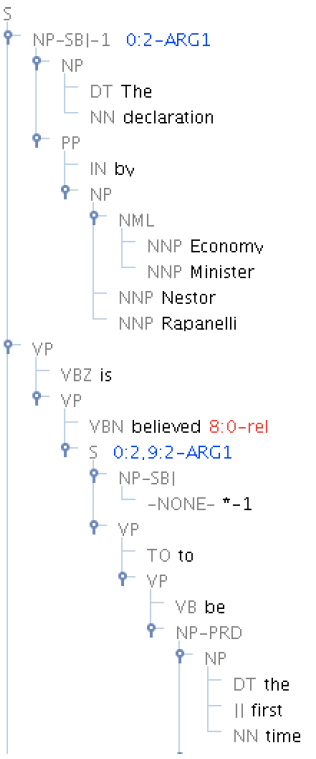
\includegraphics[scale=0.5]{img/believedex.png}}
\subfigure{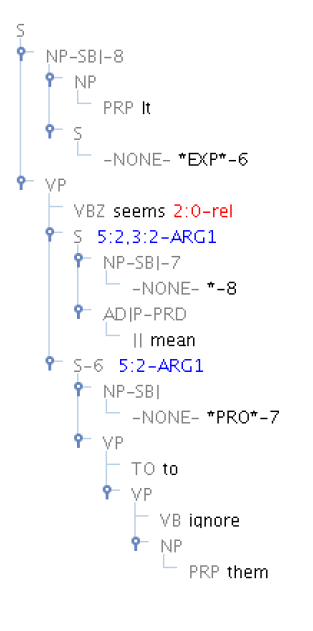
\includegraphics[scale=0.6]{img/seemex.png}}
\caption{Two Examples of Dislocated Arguments} 
\label{fig: seemex}
\end{figure}

And, finally, another class of verbs which follows this analysis includes aspectual verbs like \textit{continue} and \textit{start}, which take events as their arguments.  Watch the rolesets for these verbs carefully, often there is a separation of the aspectual sense and the agentive sense of the verb (e.g., \texttt{begin.01} and \texttt{begin.02}).  

\textit{[New loans]-4 continue [*-4] to slow.}\\
\textit{PropBank annotation:}\\
REL:	continue\\
ARG1:	[[New loans]-4] , [*-4 to slow]

\section{Handling common features of spoken data}
Annotation of transcripts of spoken data tends to be more difficult than annotation of spoken material due to disfluencies, repetitions and asides that do not normally occur in written English.  Annotation procedures for each of these types of challenges are addressed in the following sections. 

\subsection{Disfluencies and Edited Nodes}
Speakers often begin to say one utterance, stop due to a variety of speech errors or pragmatic factors, and then resume the utterance.  Sometimes the speaker resumes with a very similar utterance, other times the speaker resumes with what seems to be an entirely different utterance.  The Treebank handles such disfluencies with the use of a separate node, generally labeled \texttt{Edited}, such that the error portion of the utterance is separated from the remainder of the utterance within this node.  If the relation is not within the edited node, simply ignore edited nodes and do not annotate them, regardless of whether or not they are within the span of annotation.  If the relation is within the edited node, annotate in accordance with the normal span of annotation, but do not annotate anything past the cut off point of the utterance (this will often have a function tag in the TreeBank \texttt{UNF}, indicating that the utterance is unfinished).  In other words, treat everything before the speaker stops and switches the progression of the utterance as you normally would any relation; however, do not annotate anything beyond where the speaker stops the original utterance and then starts the repaired utterance.  See Figure~\ref{fig: Disfluency} for an example of proper annotation.  

\begin{figure}[htbp]
\centering
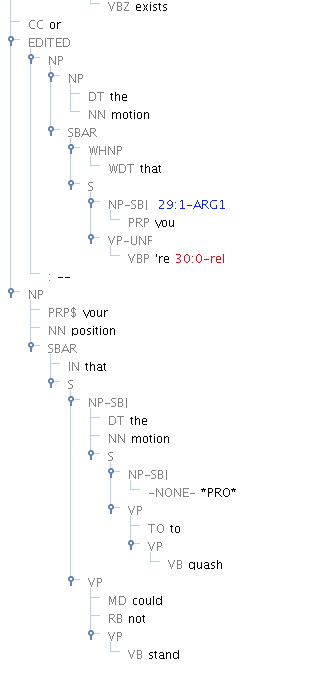
\includegraphics[scale=0.4]{img/Disfluency.png}
\caption{Correct annotation of disfluency in an edited node}
\label{fig: Disfluency}
\end{figure}

This example brings to light several common challenges in annotating disfluencies.  Notice in this example that the TreeBankers have assessed the portion of the utterance that is later repaired, and this `error' portion is placed in an edited node.  The argument of \textit{be} prior to the cut off is annotated as usual.  However, the beginning of the relative clause construction is not annotated; this is omitted because there is no index on the relativizer \textit{that} as there normally would be, which is always linked to a trace somewhere in the rest of the utterance.  As a result, there is no anchor within the clause for the relative clause construction, and it is therefore incomplete and shouldn't be annotated.  Conversely, if the trace linked to the relativizer were present within the edited node, it would require normal annotation.  Although the entire instance is not shown here, it is also notable that there is no way for the annotator to know precisely which sense to use because the utterance is incomplete.  When possible, try to use context to make the best guess of what sense of the verb is appropriate.  It is often helpful to consider the repaired utterance after the cut off because speakers sometimes continue with a very similar utterance.  However, in cases such as this one, where there is little relevant context to this portion of the utterance and the repaired utterance seems very different from the cut off utterance, simply select the most frequent sense of the verb.  The most frequent sense of the verb should be the \texttt{.01} sense; however, most of the \texttt{.01} senses in PropBank were established during annotation of the Wall Street Journal.  Thus, when tackling a very different corpus that is a transcription of spoken data, it is possible that another sense of the verb will be particularly prevalent in that corpus.  In these cases, annotators should use their best judgment of the patterns of that corpus to select what is the most likely sense of the verb in ambiguous cases.  

\subsection{Asides: PRN nodes}
In both writing and perhaps somewhat more frequently in spoken discourse, speakers may insert an utterance that is not directly related to the main utterance in progress: `\textit{It is the livestock sector, according to a new report by the United Nations Food and Agriculture Organization, that generates more greenhouse gases than any other industry.}'  In the preceding utterance, the `\textit{according to}' phrase would be encompassed in a node labeled \texttt{PRN} (meaning parenthetical) in the TreeBank.  Like \texttt{Edited} nodes, \texttt{PRN} nodes should not be annotated unless the relation is within the parenthetical node itself.  Annotation within the \texttt{PRN} node should be restricted to the normal span, meaning that it will not extend beyond the \texttt{PRN} node.  In the case of spoken discourse, such nodes are often used for embedded phrases such as `\textit{I think},' `\textit{You know},' or repair initiators such as `\textit{I mean}.'  

\chapter{Light Verb Annotation}
\label{ch: LVC}
Light verb usages are those which are considered semantically bleached, thus they do not carry the specificity of meaning that the verb would carry outside of a light verb construction~\cite{butt-93}.  For example, a `heavy' version of the verb \textit{make} is used in the phrase `\textit{She made a pie out of fresh cherries and refrigerated dough}.'  This usage reflects the normal semantic roles associated with the creation sense of \textit{make}: Agent, Product and Material.  A light version of the verb \textit{make} is used in the phrase `\textit{She made an offer to buy the company for 2 million dollars}.'  Unlike the first phrase, the verb \textit{make} does not specify the semantics of the event; rather, the eventive noun or true predicate \textit{offer} specifies the event.  For this reason, we can often rephrase light verb constructions with the verb counterpart of the eventive noun (if one exists, this is not always the case) without losing the meaning of the utterance: `\textit{She offered to buy the company}.'  In addition to specifying the semantics of the event, the eventive noun also projects the argument structure of the utterance.  For example, the infinitival complement `\textit{to buy the company}' and the price argument `\textit{for 2 million dollars}' are canonical types of arguments for \textit{offer}, but not for the verb \textit{make}: `\textit{\**She made to buy the company}.'  Similarly, the canonical arguments of the heavy sense of \textit{make} are not compatible with \textit{offer}: `?\textit{She made the offer out of intentions, ink and paper}.' Because the verb in these cases is not the element that specifies the semantics of the event or projects the argument structure, we cannot treat light verbs in the same way that we treat `heavy' verbs.  Therefore, we have special annotation procedures for light verbs, outlined in the following sections. 

\section{Pass 1: Verb Pass}
Common light verbs in English are \textit{make}, \textit{take}, \textit{get}, \textit{give}, \textit{have}, and \textit{do}, found in light verb constructions such as `\textit{John made an inspection of the premises},' `\textit{John took a walk to the store},' `\textit{John had a drink of iced tea},' and `\textit{John did an investigation of the crime}.'  The verb \textit{give} is often cited as a light verb in English as well; however, for the purposes of PropBank, \textit{give} was not originally treated as a light verb because all light verb usages of \textit{give} maintain the canonical transfer semantics and ditransitive argument structure: `\textit{She gave him thunderous applause}.'  Nonetheless, for symmetry in the events identified in sentences such as `\textit{She gave the baby a bath}' and `\textit{She took a bath},' current annotation procedures recognize \textit{give} as a light verb where its semantics are overshadowed by that its eventive or stative noun complement.  Unlike \textit{give}, most other light verbs do not maintain their canonical semantics or argument structure when used in light verb constructions.  It is theoretically possible for many other verbs to be light in certain usages, such as `\textit{She produced an alternation}.'  Whenever a verb seems to describe the event semantics less than the accompanying eventive or stative noun, it is likely a light verb construction.  In particular, annotators should consider near synonyms of the light verbs (e.g., \textit{have-possess, make-create, give-emit, get-undergo, do-execute}) to be light when they also accompany an eventive or stative noun carrying the bulk of the semantics.   

When a light verb is encountered, the annotator should perform the following steps:

\textit{Step 1: Roleset selection}\\
Annotators should select the \texttt{.LV} roleset, available for all verbs, when the verb is found in a light verb construction.  In some cases, placeholder numbered rolesets are available for light verbs.  Do not use this numbered roleset, always use the \texttt{.LV} roleset.  

\textit{Step 2: Annotation}\\
Annotators should annotate only the eventive noun or true predicate itself as ARGM-PRR (PRedicating Relation). Unlike normal tag placement, the ARGM-PRR tag should be placed directly on the lexical level or leaf containing the action nominal complement. Figure~\ref{fig: LightVerbAnnots} illustrates correct annotation of light verb constructions: 

\begin{figure}[htbp]
\centering
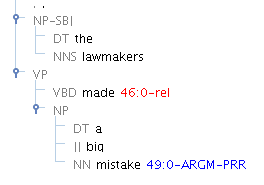
\includegraphics[scale=0.5]{img/LightVerbAnnots.png}
\caption{Correct annotation of a light verb construction}
\label{fig: LightVerbAnnots}
\end{figure}

Annotate \textbf{only} this element.  The first pass is strictly an identification pass meant to find and label light verbs as such.  We do not annotate additional arguments because the verb itself is not the relation that is projecting the argument structure; thus it is not appropriate to annotate other arguments as if they were truly semantically related to the verb.  Rather, the surrounding arguments are annotated during the second pass, when the action nominal complement is annotated, because it is the action nominal complement that projects the argument structure.  

It is often difficult to decide if a certain usage is a light verb usage or not.  Light verbs are thought to exist on a continuum ranging from the purely compositional meanings stemming from ordinary collocation of words (e.g. `\textit{I tripped on the rug}'), wherein every word maintains its full semantic value, to the entirely non-compositional meanings stemming from fixed idiomatic expressions (e.g. `\textit{I tripped the light fantastic},' meaning `\textit{to dance}').  As a result, there are often fuzzy boundaries between heavy usages of verbs, light usages of verbs, and idiomatic usages of verbs.  For the purposes of PropBank, annotators should be generous in their definition of light verb constructions and annotate accordingly when in doubt as to whether something is a light verb or not.  In turn, cases where the annotator seems to have been too generous in this definition will be corrected in adjudication. Here are several short heuristics for when to annotate an instance as \texttt{.LV}: 

\begin{enumerate}
\item Does the noun object denote an event or state? If not, it is not a light verb.  If so, proceed to next question. 

\item Are the arguments of both the noun and the verb more representative of typical arguments of the verb relation or the noun relation (e.g. `\textit{I took a walk \textbf{to the park}}')? If arguments are more typical of the verb relation, it is not a light verb.  If arguments are typical of the noun relation, proceed to next question.

\item Similarly, does the potential light verb link the eventive or stative noun to one of its typical semantic roles, realized by the subject of the verb? (e.g., `[\textit{I}]$_{AGENT}$ \textit{made a call to the hospital},' `[\textit{I}]$_{RECIPIENT}$ \textit{got a call from the hospital}').

\item Consider rephrasing the instance using a lexical verb related to the noun if one exists (e.g., `\textit{He walked to the park},' `\textit{I called the hospital},' `\textit{I was called by the hospital}'). If the rephrasing still captures the majority of the event semantics (even if there are small variations in voice, aspect or tone), then mark the instance as a light verb. Only if the verb adds semantics beyond what is captured by the eventive or stative noun should it be considered heavy.  For example, `\textit{I got a call from him}' should be considered a light verb, while `\textit{I need a call from him}' should not.  
\end{enumerate}

\section{Pass 2: Noun Pass}
The bulk of the annotation of light verb constructions will be performed during the second noun pass, wherein the action nominal complement or true predicate is the relation.  Unlike ordinary noun annotation described in Chapter~\ref{chap: Noun Annotation Instructions}, annotation of nouns that are true predicates within a light verb construction requires the annotation of arguments within both the noun relation's span of annotation (sisters to the noun and sisters to the noun phrase), and the light verb's span of annotation (sisters to the verb and sisters to the verb phrase).  In the case of light verb constructions, the syntactic arguments of both the light verb and the action nominal complement are annotated together because it is thought that both contribute to complex predication.  After identifying the fact that the noun relation is a true predicate in a light verb construction, proceed with the following steps:

\textit{Step 1: Roleset Selection}\\
Roleset selection proceeds exactly as it does for normal annotation of noun relations: select the appropriate numbered roleset according to the sense of the usage.  

\textit{Step 2: Annotation}\\
Annotate direct arguments of the noun relation (sisters to the noun and sisters to the noun phrase) and the syntactic arguments of the light verb (sisters to the verb and sisters to the verb phrase) in accordance with the argument structure outlined in the selected roleset.  In addition, annotate the light verb itself using the ARGM-LVB tag, place this tag directly on the leaf node of the light verb.  For example:

\textit{Yesterday, Mary made an accusation of duplicity against John because she was enraged with jealousy.}\\
ARGM-TMP: Yesterday\\
ARG0: Mary\\
ARGM-LVB: made\\
REL: accusation\\
ARG2: of duplicity\\
ARG1: against John\\
ARGM-CAU: because she was enraged with jealousy.

Thus, all arguments of the complex predicate (in this case make+accusation) are annotated in accordance with the true predicate's argument structure, outlined in the noun relation's roleset. 


\section{Examples}
Here is a list of examples of less typical light verb constructions: 
\begin{enumerate}
\item \textit{He got a sense of his soul.}\\
ARG0: He\\
ARGM-LVB: got\\
REL: sense\\
ARG1: of his soul

\item \textit{He does have a prior conviction for the knifepoint rape.}\\
ARG1: He\\
ARGM-LVB: have\\
ARGM-TMP: prior\\
REL: conviction\\
ARG2: for the knifepoint rape

\item \textit{Officials got a tip ICH-1 back then [that someone may have dumped the equipment]-1.} \\
ARG1: Officials\\
ARGM-LVB: got\\
REL: tip\\
ARG2: *ICH*-1 (that someone may have dumped the equipment)\\
ARGM-TMP: back then

\item \textit{*PRO* have some fun.}\\
ARG0: *PRO*\\
ARGM-LVB: have\\
REL: fun

\item \textit{You get the US attention.}\\
ARG1: You\\
ARGM-LVB: get\\
ARG0: US\\
REL: attention

\item \textit{I had no right to print that.}\\
ARG1: I\\
ARGM-LVB: had\\
ARGM-NEG: no\\
REL: right\\
ARG2: to print that

\item \textit{He took pride in his hiding.}\\
ARG0: He\\
ARGM-LVB: took\\
REL: pride\\
ARG1: in his hiding

\item \textit{We get a different excuse for this every time.}\\
ARG3: We\\
ARGM-LVB: get\\
ARGM-ADJ: different\\
REL: excuse\\
ARG1: for this\\
ARGM-TMP: every time

\item \textit{Charter schools are having some successes in this area.}\\
ARG0: Charter schools\\
ARGM-LVB: having\\
REL: successes\\
ARG1: in this area

\item \textit{China gives that impression to the world.}\\
ARG0: China\\
ARGM-LVB: gives\\
REL: impression\\
ARG1: to the world
\end{enumerate}

Each of the instances given above could be considered a somewhat `unusual' LVC, and therefore somewhat difficult to identify, for the following reasons: 1) the eventive or stative noun may not have a clear verbal counterpart, so it is hard to rephrase with a lexical verb to get a sense of what the event really is, 2) the subject argument linked by the verb is not an agent, and may be something as peripheral as a listener or recipient, 3) the light verb may seem to change the event's valency, similar to a passive voice construction.  Despite these unique characteristics, each of the above instances should be annotated as an LVC.  

\section{Tricky Cases}
There are also tricky cases of verbs being used in an abstract way with a noun complement that is eventive or stative that should \textbf{not} be annotated as LVCs.  Generally, these can be distinguished from LVC cases because the subject argument linked by the verb does \textbf{not} denote one of the eventive or stative noun's normal semantic roles. Here are a few examples: 

\begin{enumerate}
\item \textit{We've \textbf{had assassinations} before this.}\\
Note: Here, \textit{We} does not denote the person assassinated or the killer, but rather just the group of people affected by the assassinations.  The best roleset for this case would be \texttt{have.03}, indicating abstract possession.  

\item\textit{*PRO* \textbf{give} us your \textbf{assessment}.}\\
Note: Here, the semantics of transfer overshadow the semantics of \textit{assessment}, as indicated by the fact that the recipient, \textit{us}, does not denote an argument that's part of the normal \textit{assessment} roleset.  Because the transfer semantics are strong for the above example, the best roleset would be \texttt{give.01}.  For light cases of \textit{give}, what can be thought of as the Recipient in terms of verb semantics is often the patient in terms of the eventive or stative noun semantics: `\textit{He gave his opponent a quick jab},' i.e., `\textit{He quickly jabbed his opponent}.'  In other cases, the Recipient in terms of verb semantics is also a recipient in terms of the eventive or stative noun's semantics, but importantly, in these cases the noun's roleset includes a recipient of some sort, such as a listener: `\textit{The president gave a rousing speech to the class of 2010}.'

\item\textit{It \textbf{gives} you a \textbf{sense} of the terror she must have felt.}\\
Note: Here, \textit{give} introduces an outside causer that is not part of the eventive noun's roleset (something is causing you to sense something).  Since a sense of what she felt is being metaphorically transferred or imparted, the best roleset is \texttt{give.01}. Similarly, `\textit{You gave me the ride of my life}' introduces an outside causer of the \textit{ride} that is not part of the normal \textit{ride} roleset. 
\end{enumerate} 

The common thread here is that although the verb is potentially light and is accompanied by an eventive or stative noun, it should not be annotated as an LVC because the verb is not acting as part of a complex relation to syntactically link the eventive or stative noun to the subject argument. 

The usages of \textit{give} that introduce an outside causer bring up the related fact that verbs whose lexical semantics include causation, such as \textit{cause} or \textit{make} should also not be annotated as light verbs, even where they happen to link an eventive or stative noun complement to a potential Agent/Cause ARG0: `\textit{The failing economy caused the end of the industry}.'  Although in many ways this case does fit the definition of a light verb (`\textit{the failing economy}' can be seen as an agent of \textit{end}: `\textit{The failing economy ended the industry}'), because causation is part of the primary semantics of the verb \textit{cause}, it is more consistent to consider these arguments to be primarily projected by the verb rather than the eventive noun, and therefore forego annotation as a light verb. 

\chapter{Noun Annotation Instructions}
\label{chap: Noun Annotation Instructions}
Nouns can also be relations in the same way that verbs are often relations.  Nominalizations and eventive nouns are especially likely to have an argument structure similar to that of a verb.  For example, `\textit{The troops' destruction of the city},'  can be thought of as the nominal counterpart of the clause `\textit{The troops destroyed the city}.'  Thus, PropBank treats certain nominalizations and eventive nouns as relations to be annotated in the same manner as verb annotations: 1) select the appropriate roleset created specifically for the noun relation, 2) annotate numbered arguments in accordance with this roleset, and 3) annotate modifier arguments with the appropriate ARGM tags.  However, there are a few differences to be aware of when annotating nouns, which are outlined in the following sections.  

\section{Span of Annotation}
The span of annotation for noun relations mirrors that of verb relations.  Instead of annotating the sisters to the verb and sisters to the verb phrase, annotation is required for the sisters to the noun and sisters to the noun phrase that encompasses the noun relation.  Figure~\ref{fig: NounSpan} illustrates the noun relation's span of annotation.  Also like the verb span of annotation wherein several VP nodes may encompass a verb, several NP nodes may encompass the noun relation, and arguments of the noun relation to be tagged can be sisters to each of these NP nodes.  In the case of verbs, the annotator can use the position of the clause boundary to determine where the span of annotation is delimited.  However, in the case of nouns, the boundary of the span is marked by another NP (or occasionally NOM) node.  Annotators must determine which NP node is the stopping point by finding which is a sister to the verb.  Annotators cannot annotate sisters to the highest NP node that is a sister to the verb because this will entail annotating sisters to the verb itself.  This is illustrated in Figure~\ref{fig: EmbeddedNPs}. The long arrows indicate valid arguments of the noun relation, while the top T indicates the sister to the highest NP node, which is a sister to the verb \textit{is}, thus, annotators should consider this NP node as the stopping point for annotation.  

\begin{figure}[htbp]
\centering
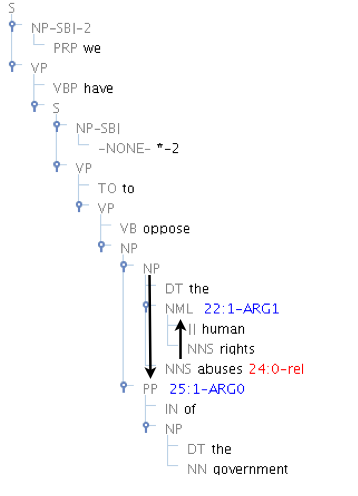
\includegraphics[scale=0.5]{img/NounSpan.png}
\caption{Noun span of annotation: the arrow to the right points to the sister of the noun, and the arrow to the left points to the sister of the noun phrase encompassing the noun relation}
\label{fig: NounSpan}
\end{figure}

\begin{figure}[htbp]
\centering
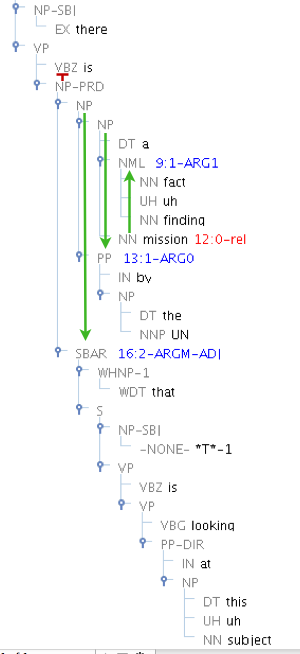
\includegraphics[scale=0.5]{img/EmbeddedNPs.png}
\caption{Noun span of annotation: the arrows point to arguments of the noun relation that should be tagged, while the highest NP node with the `T' above it indicates the delimiting node of the span}
\label{fig: EmbeddedNPs}
\end{figure}

\pagebreak

In the case of a list of nouns ([NP and NP], [NP but not NP], [NP, NP, and NP], and so on), the span of annotation does not extent to list items other than the one containing the Rel. Figure~\ref{fig: list} shows an example of correct list annotation. 

\begin{figure}[htbp]
\centering
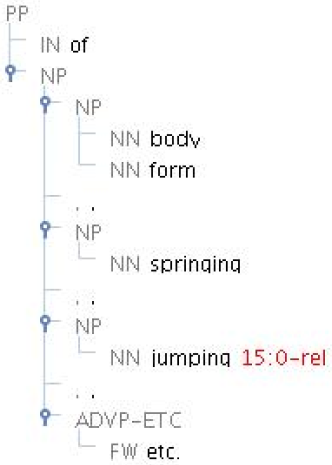
\includegraphics[scale=0.5]{img/list.png}
\caption{Noun List Annotation}
\label{fig: list}
\end{figure}

\section{Annotation of Numbered Arguments}
Numbered arguments for noun relations are outlined in the corresponding noun frame file and rolesets therein.  These should be selected in Jubilee in the same manner as verb rolesets.  It is important to keep in mind that the type and order of constituents is highly variable for noun relations.  For example, both agents and patients can appear before the relation as a possessor or noun modifier, or in a prepositional argument after the relation. 

\textit{Channel Nine's broadcast of the nightly news was praised for its quality.}\\
ARG0: Channel Nine's\\
REL: broadcast\\
ARG1: of the nightly news

\textit{The nightly news broadcast of Channel Nine was praised for its quality.}\\
ARG1: nightly news\\
REL: broadcast \\
ARG0: of Channel Nine

As a result of this variability, it is especially important to think of the primary goal of PropBank when annotating noun relations: assign the appropriate semantic tag across various syntactic realizations of the argument. 

\section{Annotation of Modifiers}
Modifier arguments are identical for nouns with one exception, the ARGM-ADJ tag described below.  That which is often expressed as adverbs in the case of verb relations is expressed with adjectives for noun relations: 

\textit{Was your personal experience of having been on the cruise pleasurable?}\\
ARG0: your\\
ARGM-MNR: personal\\
REL: experience\\
ARG1: of having been on the cruise

In the above example, one can think of \textit{personal} as equivalent to \textit{personally} in the clause counterpart of the phrase: `\textit{You personally experienced having been on the cruise}.'  If it is helpful, try to rephrase the instance in this manner to decide what type of argument it would be when accompanying a verb, and it will be the same type of modifier when accompanying the noun relation. 

\subsection{Adjectival modifiers (ADJ)}
\label{ssec: ADJ}

Instead of the modifier tag ADV, which should never be used for noun relations, the modifier tag ARGM-ADJ is used to label arguments that cannot be appropriately labeled with any other ARGM tag.  As with the ARGM-ADV tag, the ARGM-ADJ tag should only be used as a last resort, when no other argument label can possibly fit.  For example: 

\textit{The mayor's shocking abuse of public funds outraged citizens.}\\
ARG0: The mayor's\\
ARGM-ADJ: shocking\\
REL: abuse\\
ARG1: of public funds

In the above example, the manner of the abuse is not shocking, `?\textit{he shockingly abused public funds};' rather, the entire event is perceived as shocking by outsiders.  Its verb counterpart would be something akin to `\textit{Shockingly, the mayor abused public funds},' and would be annotated as ARGM-ADV for lack of a better tag.  Similarly, modifiers such as this must be tagged as ARGM-ADJ for lack of a more specific tag.  \texttt{SBAR} modifiers, as seen in Figure~\ref{fig: EmbeddedNPs} should also be tagged as ARGM-ADJ, along with quantity phrases, such as Figure~\ref{fig: quantity}.

\begin{figure}[htbp]
\centering
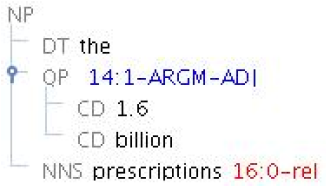
\includegraphics[scale=0.4]{img/quantity.png}
\caption{An Example of Adjectival Quantity}
\label{fig: quantity}
\end{figure}

\subsection{Secondary Predication modifiers (PRD)}
\label{ssec: PRDnouns}
In noun annotation, verbal modifiers of the \texttt{rel} are considered secondary predication because they are eventually annotated as well. Figure~\ref{fig: nounPRD} shows two instances of secondary predication in noun annotation. An important distinction in `\textit{\ldots a judgement based on the law}' is that the \texttt{VP} is only included in the span of annotation because of the NP mother node encompassing both the \texttt{NP} containing the \texttt{rel} and the \texttt{VP} itself. If the mother \texttt{NP} was an \texttt{S} node, the \texttt{VP} would not be included in the span of annotation. 

\begin{figure}[htbp]
\centering
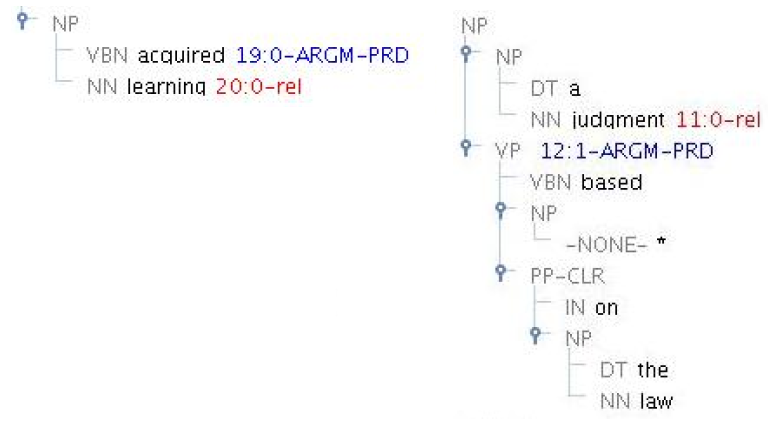
\includegraphics[scale=0.374]{img/nounprd.png}
\caption{An Example of Secondary Predication in Noun Annotation}
\label{fig: nounPRD}
\end{figure}

\section{Exceptions to Annotation: Determiners and Other Noun Relations}
As with verb annotation, the articles \textit{a}, \textit{an}, and \textit{the} should not be annotated when they are in the span of annotation for a noun relation, nor should the majority of other determiners (\textit{this}, \textit{that}, \textit{some}, \textit{any}, etc.), labeled \texttt{DT} in the Treebank.  The greatest exception to this is, of course, possessive determiners which frequently correspond to numbered arguments.  Additionally, certain determiners such as \textit{first} and \textit{final} can be annotated as ARGM-TMP when they denote the time or frequency of the event.  Finally, negative determiners \textit{no}, and \textit{neither} should be tagged as ARGM-NEG.  

Just as we do not annotate other coordinated verbs that fall within the span of annotation of a given verb relation, we do not annotate other coordinated eventive nouns or nominalizations that fall within the span of annotation of a given noun relation.  For example:

\textit{Mary's investigation and eventual condemnation of the local government made the news.}\\
ARG0: Mary's\\
ARGM-TMP: eventual\\
REL: condemnation\\
ARG1: of the mayor

Outside of these exceptions, all other arguments within the span of annotation should be annotated.  

\section{.YY Roleset}
\label{sec: YYrole}

In some instances, there are nouns which come up for annotation which should not be annotated. These cases include:\par
1) Non-eventive nouns \\
\hspace*{10 mm} A noun must denote an event or a state. Eventive nouns are always abstract, not concrete, but not all abstract nouns are eventive. For example, \textit{building} in the sentence `\textit{The building on the left\ldots}' refers to a concrete entity and should not be annotated, while \textit{building} in the sentence `\textit{The building of the Eiffel Tower many years ago}' refers to an abstract event and should be annotated. Figure~\ref{fig: nenouns} shows further examples of the difference. \par

\begin{figure}[htbp]
\centering
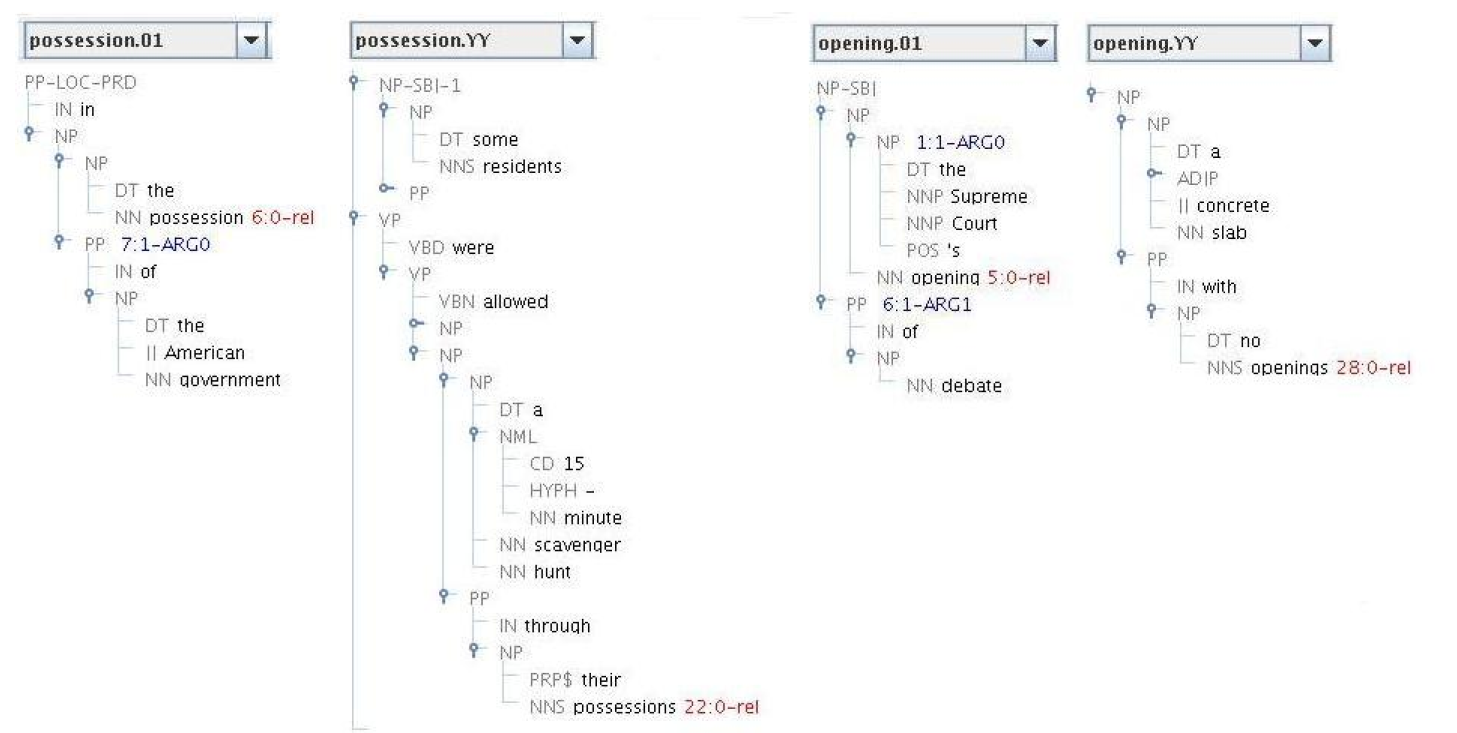
\includegraphics[scale=0.4]{img/nenouns.png}
\caption{An Example of Non-Eventive Nouns (\texttt{.YY}) and Eventive Nouns}
\label{fig: nenouns}
\end{figure}

2) Non-head nouns \\
\hspace*{10 mm} A noun \texttt{rel} must be a head, or a final noun in any noun-noun compound. The head noun is the noun which projects argument structure. Any noun which comes up for annotation which is not a head noun should not be annotated, but marked with the \texttt{.YY} roleset. Figure~\ref{fig: headnouns} shows an example of a head versus non-head noun \texttt{rel} distinction. In the instance marked as \texttt{.YY}, the \texttt{rel} \textit{jumping} is not the head noun; the noun "\textit{jumping}" modifies the head of the noun phrase, "\textit{portion}". The instance marked \texttt{learning.01} shows a head noun in an unusual position (where a modifier is expected). 

\begin{figure}[htbp]
\centering
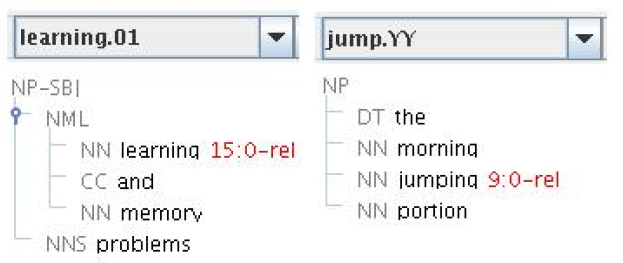
\includegraphics[scale=0.4]{img/headnouns.png}
\caption{An Example of Head Nouns and Non-Head Nouns (\texttt{.YY})}
\label{fig: headnouns}
\end{figure}

\chapter{Adjectival Predicate Annotation Instructions}
\label{ch: ADJ Annotation}
Crosslinguistically, it is common for there to be overlap between what is expressed as a verb and what is expressed as an adjective.  Even in English, it can be difficult to distinguish between copular constructions and auxiliaries (e.g. `\textit{He is limited/balding}').  In other languages, what would be considered an adjective in English may be expressed as a verb (given evidence from verbal morphology); for example, in Lakota, `\textit{I am thirsty}' would be expressed with the stative verb \textit{\'{i}mapuze}.  Because PropBank is in part a resource for machine translation and several parallel PropBanks exist in different languages, it is important to annotate predicate adjectives in English.  

\section{Span of Annotation}
The span of annotation for adjectives is very similar to that of the noun pass in LVC annotation.  Because nouns require the support of a verb to express arguments, the predicate adjective and support verb together form what can be thought of as a complex predicate.  Unlike LVC annotation, there is no special tag for the copular, or support, verb itself.  However, annotation is required for sisters of the adjectival predicate (marked \texttt{JJ} in the Treebank) itself, sisters to the adjectival phrase that contains the predicate (\texttt{ADJP}), sisters to the support verb (with the exception of the \texttt{ADJP} sister itself; tagging this will cause recursive annotation since the \texttt{ADJP} contains the \texttt{JJ} and potentially other arguments), and sisters to the \texttt{VP(s)} that contains the support verb.  An image of correct adjective annotation is given in Figure~\ref{fig: AdjSpan}.  

\begin{figure}[htbp]
\centering
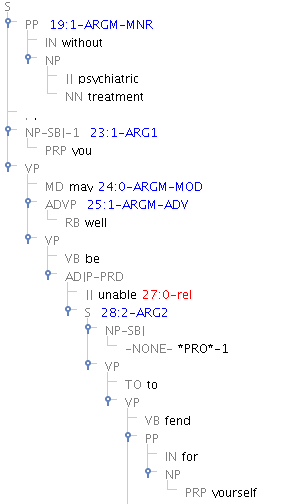
\includegraphics[scale=0.5]{img/AdjSpan.png}
\caption{Adjective Span of annotation: note that sisters to both the JJ predicate and the support verb are both annotated.}
\label{fig: AdjSpan}
\end{figure}

\section{Annotation of Arguments}
Annotation of numbered arguments follows the adjectival predicate's roleset, as in both noun and verb annotation.  Annotation of ARGMs proceeds in exactly the same manner as verb annotation (not noun annotation: the ADJ and LVB tags will not be used; the ADV tag is used).  Additionally, exceptions to annotation (e.g., determiners or coordinated adjectival predicates) will also be followed as outlined for verb annotation.  

\section{Annotating Constructions}
Essentially all gradable adjectives can participate in degree and comparative patterns that license the adjective relation to take (an) extra argument(s). As evidenced by the fact that these patterns are generalizable across adjectives rather than internally dictated, arguments are likely projected by the constructions themselves, rather than the relation. In order to show this pattern, the arguments of the construction should be annotated with the Construction (CXN) marker. These CXN markers should be concatenated if and when the construction requires both parts or arguments to complete the pattern.  Currently, three frequent constructions have been identified occurring with adjective relations: the Comparative Construction, the Degree Construction, and `the Xer the Yer' Construction.  These constructions are discussed in turn below. It is, of course, possible that other annotatable constructions exist.  If it is noted that there is an argument present that is not normally projected by the semantics of the adjective relation, and instead there is a patterned phrasing (or construction) surrounding the relation that is generalizable to a variety of other relations, then annotators can use the CXN tags to mark the constructional argument.  In these cases, please take a screen shot of the potential construction and contact the annotation supervisor with details.  

\subsection{Comparative Constructions}
Comparative sentences fit a `more/less/as-X than/as Y' pattern. For example, in `\textit{Hillary Clinton is \textbf{about as} damaging to the Dem Party \textbf{as Jeremiah Wright}},' Hilary Clinton is compared to Jeremiah Wright in terms of damage done.  Correct annotation of this instance is shown in Figure~\ref{fig: ComparativeConstruction}. 
	
\begin{figure}[htbp]
\centering
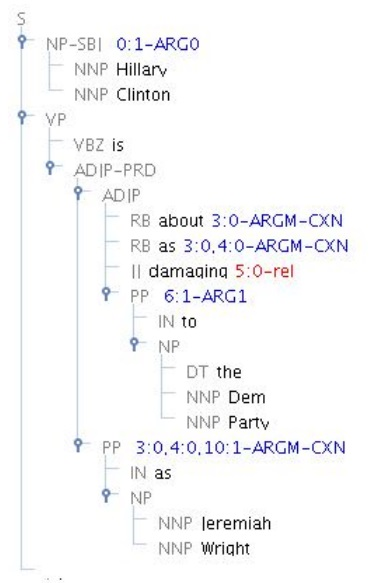
\includegraphics[scale=0.6]{img/asDamaging.jpg}
\caption{Annotation of a Compative Construction.}
\label{fig: ComparativeConstruction}
\end{figure}

All participants in the construction are tagged with the CXN marker here. Note that while both \textit{about} and \textit{as} are required to tell the degree to which she is damaging, they are not subsumed under one node. Regardless of the number of CXN markers needed to capture the entire pattern, all tags should be concatenated (see Section~\ref{sec: concatenation} to review how to concatenate arguments if necessary).  In some cases, the first comparison word (\textit{more}/\textit{less}) is lexicalized as part of the adjective relation: \textit{better, worse, taller, smarter,} etc.  In these cases, only the second portion of the construction (the \textit{than} phrase) is marked with the CXN tag.  Finally, if only the first portion of the construction is given, without a full mention of what something is being compared to, no CXN tag will be used, as there is really no argument projected by the construction in this case (e.g. `\textit{Someday, things will be better}').  

\subsection{Degree Construction}
Constructions of this type tell the degree to which something is done or a state is true, and often mention a consequence of the degree to which a state is true. These sentences complete the pattern `X is too/so Y to/that Z,' or `X is not Y enough to/that Z.'  Annotation is done the same way for degree sentences as for comparatives, with both the degree word and its counterpart (generally an infinitival or complement clause) receiving the concatenated CXN marker.  For example, in Figure~\ref{fig: DegreeConstruction}, both the degree indicator \textit{too} and its descriptive counterpart `\textit{\texttt{*PRO*} to learn}' are concatenated with the CXN marker: 

\begin{figure}[htbp]
\centering
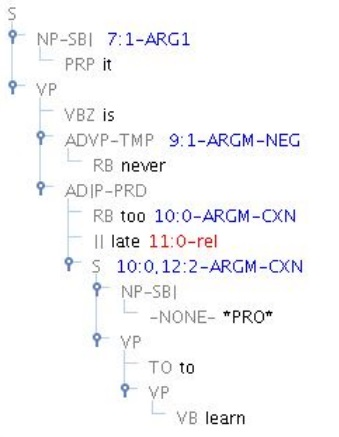
\includegraphics[scale=0.6]{img/tooLate.jpg}
\caption{Annotation of a Degree Construction.}
\label{fig: DegreeConstruction}
\end{figure}

\subsection{The Xer the Yer Construction}
A variation of the comparative construction, these constructions fit the pattern `the X-er the Y-er.'  When X and Y are concatenated here, we see a resulting state; for example, in `\textit{the longer he is around the more miserable I will be},' we are able to show that his staying longer results in a more miserable state. Correct annotation of this construction is shown in Figure~\ref{fig: XerYerConstruction}. 

\begin{figure}[htbp]
\centering
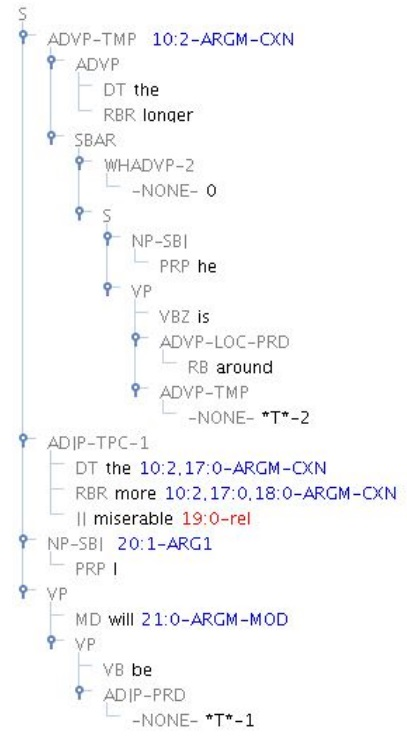
\includegraphics[scale=0.7]{img/XerYer.jpg}
\caption{Annotation of a `The Xer the Yer' Construction.}
\label{fig: XerYerConstruction}
\end{figure}

These patterns will almost always require at least three CXN markers. Also, note that the determiner \textit{the} is considered to be an integral part of this construction. 

\pagebreak
\appendix
\chapter{Jubilee Hotkeys}

These tables illustrate Jubilee's Hotkeys, along with Section references for each function. 

\begin{table}[htp]
\centering
\begin{tabular}{|c|c|c|}
\hline \multicolumn{3}{|c|}{\textbf{Basic Argument Annotation}} \\
\hline \textbf{Function} & \textbf{Hotkey} & \textbf{Reference Section} \\
\hline \tt rel & Ctrl+Shift+? & NA \\
\hline \tt Argument 0 & 0 & Section~\ref{ssec: Choosing ARG0 versus ARG1} \\
\hline \tt Argument 1& 1 & Section~\ref{ssec: Choosing ARG0 versus ARG1} \\
\hline \tt Argument 2& 2 & Section~\ref{ssec: Argroles} \\
\hline \tt Argument 3& 3 & Section~\ref{ssec: Argroles} \\
\hline \tt Argument 4& 4 & Section~\ref{ssec: Argroles} \\
\hline \tt Argument 5& 5 & Section~\ref{ssec: Argroles} \\
\hline \tt Argument A & A & Section~\ref{ssec: ARGA} \\
\hline \tt Comitative & 8 & Section~\ref{ssec: COM} \\
\hline \tt Locative & L & Section~\ref{ssec: LOC} \\
\hline \tt Directional & D & Section~\ref{ssec: DIR} \\
\hline \tt Goal & G & Section~\ref{ssec: GOL} \\
\hline \tt Manner & M & Section~\ref{ssec: MNR} \\
\hline \tt Temporal & T & Section~\ref{ssec: TMP} \\
\hline \tt Extent & E & Section~\ref{ssec: EXT} \\
\hline \tt Reciprocals & 9 & Section~\ref{ssec: REC} \\
\hline \tt Secondary Predication & 7 & Section~\ref{ssec: PRD} \\
\hline \tt Purpose & P & Section~\ref{ssec: PRP} \\
\hline \tt Cause & C & Section~\ref{ssec: CAU} \\
\hline \tt Discourse & I & Section~\ref{ssec: DIS} \\
\hline \tt Adverbials & V & Section~\ref{ssec: ADV} \\
\hline \tt Adjectival & J & Section~\ref{ssec: ADJ} \\
\hline \tt Modal & O & Section~\ref{ssec: MOD} \\
\hline \tt Negation & N & Section~\ref{ssec: NEG} \\
\hline \tt Direct Speech & S & Section~\ref{ssec: DSP} \\
\hline \tt Light Verb & B & Section~\ref{ssec: LVB} \\
\hline \tt Erase Annotation & - & NA \\
\hline 
\end{tabular}
\label{tbl: JubHotkeys1}
\caption{Common Jubilee Hotkeys}
\end{table} 

\pagebreak

\begin{table}[htp]
\centering
\begin{tabular}{|c|c|c|}
\hline \multicolumn{3}{|c|}{\textbf{Concatenation, Null Elements, Traces}} \\
\hline \textbf{Function} & \textbf{Hotkey} & \textbf{Reference Section} \\
\hline Link Null Element with Coreferential Argument & Ctrl+Shift+8 & Sections~\ref{sec: null1},~\ref{sec: null2} \\
\hline Concatenate Arguments & Ctrl+Shift+, & Sections~\ref{sec: null1},~\ref{sec: null2} \\
\hline Link Unindexed Object (Reduced Relative only) & Ctrl+Shift+7 & Sections~\ref{sec: null1},~\ref{sec: null2} \\
\hline Reset Rel or Concatenate Verb Particles & Ctrl+Shift+/ & Sections~\ref{sec: null1},~\ref{sec: null2} \\
\hline \multicolumn{3}{c}{} \\
\hline \multicolumn{3}{|c|}{\textbf{Toolbar and Other Functions}} \\
\hline \textbf{Function} & \textbf{Hotkey} & \textbf{Reference Section} \\
\hline \tt File > Open & Ctrl+O & NA \\
\hline \tt File > Save & Ctrl+S & NA \\
\hline \tt File > Quit & Ctrl+Q & NA \\
\hline \tt Treebank > Previous Tree & Comma & NA \\
\hline \tt Treebank > Next Tree & Period & NA \\
\hline \tt Treebank > Jump to ... & Ctrl+J & NA \\
\hline \tt Treebank > View Tree in Text & Ctrl+T & NA \\
\hline \tt Treebank > View Tree in Context & Ctrl+Shift+O & NA \\
\hline \tt Frameset > Previous Roleset & [ & NA \\
\hline \tt Frameset > Next Roleset & ] & NA \\
\hline \tt Frameset > View Examples & Ctrl+E & NA \\
\hline \tt Frameset > View Arguments & Ctrl+W & NA \\
\hline \tt Frameset > View Roleset Comments & Ctrl+C & NA \\
\hline \tt Help > About & F1 & NA \\
\hline 
\end{tabular}
\label{tbl: JubHotkeys2}
\caption{Concatenation, Null Elements, Traces, and Toolbar Function Hotkeys}
\end{table} 

\pagebreak

\addcontentsline{toc}{chapter}{References}
\bibliography{references}
\end{document}  
